\INEchaptercarta[Fecundidad y planificación familiar]{Características escolares de las mujeres en edad fértil}{}



\cajita{TGF}{La tasa global de fecundidad, según la encuesta nacional de salud materno infantil 2008-09, ha disminuido de 5.6 hijos por mujer a 3.6.}{Tasa global de fecundidad }{República de Guatemala, serie histórica por ENSMI, niños por mujer}{\ \\[0mm]\begin{tikzpicture}[x=1pt,y=1pt]  % Created by tikzDevice version 0.7.0 on 2015-09-01 14:15:14
% !TEX encoding = UTF-8 Unicode
\definecolor[named]{fillColor}{rgb}{1.00,1.00,1.00}
\path[use as bounding box,fill=fillColor,fill opacity=0.00] (0,0) rectangle (289.08,198.74);
\begin{scope}
\path[clip] (  0.00,  0.00) rectangle (289.08,198.74);
\definecolor[named]{drawColor}{rgb}{1.00,1.00,1.00}

\path[draw=drawColor,line width= 0.6pt,line join=round,line cap=round] (  0.00,  0.00) rectangle (289.08,198.74);
\end{scope}
\begin{scope}
\path[clip] (  0.00,  0.00) rectangle (289.08,198.74);

\path[] ( -2.73, 17.78) rectangle (280.54,191.48);

\path[] (  0.00, 53.87) --
	(280.54, 53.87);

\path[] (  0.00,110.27) --
	(280.54,110.27);

\path[] (  0.00,166.67) --
	(280.54,166.67);

\path[] (  0.00, 25.67) --
	(280.54, 25.67);

\path[] (  0.00, 82.07) --
	(280.54, 82.07);

\path[] (  0.00,138.47) --
	(280.54,138.47);

\path[] ( 29.95, 17.78) --
	( 29.95,191.48);

\path[] ( 84.43, 17.78) --
	( 84.43,191.48);

\path[] (138.90, 17.78) --
	(138.90,191.48);

\path[] (193.38, 17.78) --
	(193.38,191.48);

\path[] (247.86, 17.78) --
	(247.86,191.48);
\definecolor[named]{drawColor}{rgb}{0.00,0.00,1.00}

\path[draw=drawColor,line width= 1.7pt,line join=round] ( 29.95,183.59) --
	( 84.43,169.49) --
	(138.90,166.67) --
	(193.38,149.75) --
	(247.86,127.19);
\definecolor[named]{drawColor}{rgb}{0.00,0.00,0.00}

\node[text=drawColor,anchor=base,inner sep=0pt, outer sep=0pt, scale=  1.01] at ( 29.95,187.54) {5.6};

\node[text=drawColor,anchor=base west,inner sep=0pt, outer sep=0pt, scale=  1.01] at ( 84.43,173.44) {5.1};

\node[text=drawColor,anchor=base west,inner sep=0pt, outer sep=0pt, scale=  1.01] at (138.90,170.62) {5.0};

\node[text=drawColor,anchor=base west,inner sep=0pt, outer sep=0pt, scale=  1.01] at (193.38,153.70) {4.4};

\node[text=drawColor,anchor=base,inner sep=0pt, outer sep=0pt, scale=  1.01] at (247.86,115.32) {3.6};
\definecolor[named]{fillColor}{rgb}{0.00,0.00,0.00}

\path[draw=drawColor,line width= 0.1pt,line join=round,fill=fillColor] (  0.00, 25.67) -- (280.54, 25.67);
\end{scope}
\begin{scope}
\path[clip] (  0.00,  0.00) rectangle (289.08,198.74);

\path[] (  0.00, 17.78) --
	(280.54, 17.78);
\end{scope}
\begin{scope}
\path[clip] (  0.00,  0.00) rectangle (289.08,198.74);

\path[] ( 29.95, 13.51) --
	( 29.95, 17.78);

\path[] ( 84.43, 13.51) --
	( 84.43, 17.78);

\path[] (138.90, 13.51) --
	(138.90, 17.78);

\path[] (193.38, 13.51) --
	(193.38, 17.78);

\path[] (247.86, 13.51) --
	(247.86, 17.78);
\end{scope}
\begin{scope}
\path[clip] (  0.00,  0.00) rectangle (289.08,198.74);
\definecolor[named]{drawColor}{rgb}{0.00,0.00,0.00}

\node[text=drawColor,anchor=base,inner sep=0pt, outer sep=0pt, scale=  1.00] at ( 29.95,  2.85) {1987};

\node[text=drawColor,anchor=base,inner sep=0pt, outer sep=0pt, scale=  1.00] at ( 84.43,  2.85) {1995};

\node[text=drawColor,anchor=base,inner sep=0pt, outer sep=0pt, scale=  1.00] at (138.90,  2.85) {1998/99};

\node[text=drawColor,anchor=base,inner sep=0pt, outer sep=0pt, scale=  1.00] at (193.38,  2.85) {2002};

\node[text=drawColor,anchor=base,inner sep=0pt, outer sep=0pt, scale=  1.00] at (247.86,  2.85) {2008/09};
\end{scope}
  \end{tikzpicture}}{Instituto Nacional de Estadística, con datos de la Encuesta Nacional de Salud Materno Infantil}


\cajita{TGF según escolaridad}{Según el nivel de escolaridad de las mujeres, la tasa de fecundidad en mujeres con educación superior fue de 1.7 hijos por mujer. Asimismo, 5.2 hijos por mujer es la tasa de fecundidad en las mujeres sin educación.}{Tasa global de fecundidad por nivel de educación}{República de Guatemala, 2008-09, niños por mujer}{\ \\[0mm]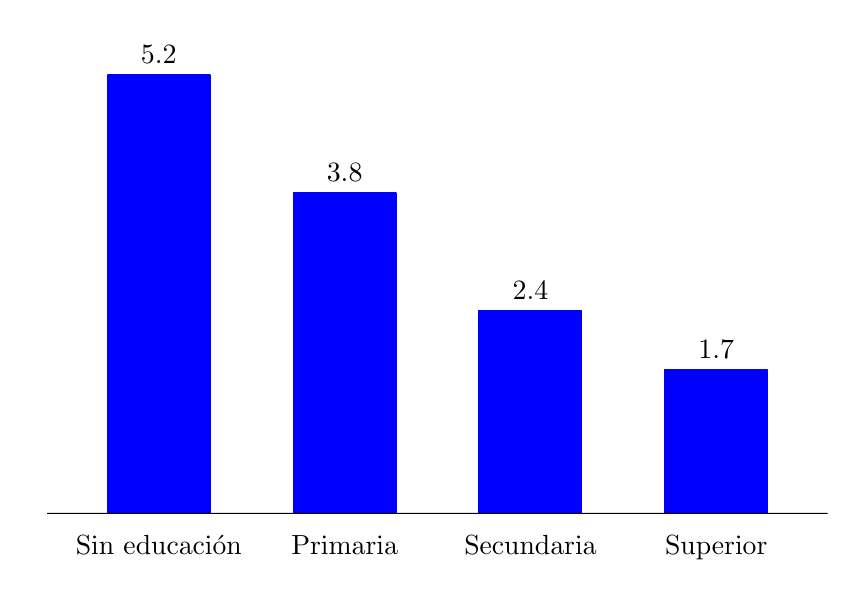
\begin{tikzpicture}[x=1pt,y=1pt]  % Created by tikzDevice version 0.7.0 on 2015-09-08 18:21:10
% !TEX encoding = UTF-8 Unicode
\definecolor[named]{fillColor}{rgb}{1.00,1.00,1.00}
\path[use as bounding box,fill=fillColor,fill opacity=0.00] (0,0) rectangle (289.08,198.74);
\begin{scope}
\path[clip] (  0.00,  0.00) rectangle (289.08,198.74);
\definecolor[named]{drawColor}{rgb}{1.00,1.00,1.00}

\path[draw=drawColor,line width= 0.6pt,line join=round,line cap=round] (  0.00,  0.00) rectangle (289.08,198.74);
\end{scope}
\begin{scope}
\path[clip] (  0.00,  0.00) rectangle (289.08,198.74);

\path[] (  7.11, 23.47) rectangle (289.08,181.67);

\path[] ( 47.39, 23.47) --
	( 47.39,181.67);

\path[] (114.53, 23.47) --
	(114.53,181.67);

\path[] (181.66, 23.47) --
	(181.66,181.67);

\path[] (248.80, 23.47) --
	(248.80,181.67);
\definecolor[named]{drawColor}{rgb}{0.00,0.00,1.00}
\definecolor[named]{fillColor}{rgb}{0.00,0.00,1.00}

\path[draw=drawColor,line width= 0.6pt,line join=round,fill=fillColor] ( 28.93, 23.47) rectangle ( 65.86,181.67);

\path[draw=drawColor,line width= 0.6pt,line join=round,fill=fillColor] ( 96.07, 23.47) rectangle (132.99,139.08);

\path[draw=drawColor,line width= 0.6pt,line join=round,fill=fillColor] (163.20, 23.47) rectangle (200.13, 96.48);

\path[draw=drawColor,line width= 0.6pt,line join=round,fill=fillColor] (230.34, 23.47) rectangle (267.26, 75.19);
\definecolor[named]{drawColor}{rgb}{0.00,0.00,0.00}
\definecolor[named]{fillColor}{rgb}{0.00,0.00,0.00}

\path[draw=drawColor,line width= 0.1pt,line join=round,fill=fillColor] (  7.11, 23.47) -- (289.08, 23.47);

\node[text=drawColor,anchor=base,inner sep=0pt, outer sep=0pt, scale=  1.01] at ( 47.39,185.63) {5.2};

\node[text=drawColor,anchor=base,inner sep=0pt, outer sep=0pt, scale=  1.01] at (114.53,143.03) {3.8};

\node[text=drawColor,anchor=base,inner sep=0pt, outer sep=0pt, scale=  1.01] at (181.66,100.44) {2.4};

\node[text=drawColor,anchor=base,inner sep=0pt, outer sep=0pt, scale=  1.01] at (248.80, 79.14) {1.7};
\end{scope}
\begin{scope}
\path[clip] (  0.00,  0.00) rectangle (289.08,198.74);

\path[] (  7.11, 23.47) --
	(  7.11,181.67);
\end{scope}
\begin{scope}
\path[clip] (  0.00,  0.00) rectangle (289.08,198.74);

\path[] (  7.11, 23.47) --
	(289.08, 23.47);
\end{scope}
\begin{scope}
\path[clip] (  0.00,  0.00) rectangle (289.08,198.74);

\path[] ( 47.39, 19.20) --
	( 47.39, 23.47);

\path[] (114.53, 19.20) --
	(114.53, 23.47);

\path[] (181.66, 19.20) --
	(181.66, 23.47);

\path[] (248.80, 19.20) --
	(248.80, 23.47);
\end{scope}
\begin{scope}
\path[clip] (  0.00,  0.00) rectangle (289.08,198.74);
\definecolor[named]{drawColor}{rgb}{0.00,0.00,0.00}

\node[text=drawColor,anchor=base,inner sep=0pt, outer sep=0pt, scale=  1.00] at ( 47.39,  8.54) {Sin educaci\'on};

\node[text=drawColor,anchor=base,inner sep=0pt, outer sep=0pt, scale=  1.00] at (114.53,  8.54) {Primaria};

\node[text=drawColor,anchor=base,inner sep=0pt, outer sep=0pt, scale=  1.00] at (181.66,  8.54) {Secundaria};

\node[text=drawColor,anchor=base,inner sep=0pt, outer sep=0pt, scale=  1.00] at (248.80,  8.54) {Superior};
\end{scope}
  \end{tikzpicture}}{Instituto Nacional de Estadística, con datos de la Encuesta Nacional de Salud Materno Infantil}


\cajita{TGF mujeres sin educación}{Según la encuesta nacional de salud materno infantil, el número de hijos por mujer sin educación ha disminuido de 7.1 a 5.2.}{Tasa global de fecundidad de las mujeres sin educación}{República de Guatemala, serie histórica por ENSMI, niños por mujer}{\ \\[0mm]\begin{tikzpicture}[x=1pt,y=1pt]  % Created by tikzDevice version 0.7.0 on 2015-09-01 14:15:59
% !TEX encoding = UTF-8 Unicode
\definecolor[named]{fillColor}{rgb}{1.00,1.00,1.00}
\path[use as bounding box,fill=fillColor,fill opacity=0.00] (0,0) rectangle (289.08,198.74);
\begin{scope}
\path[clip] (  0.00,  0.00) rectangle (289.08,198.74);
\definecolor[named]{drawColor}{rgb}{1.00,1.00,1.00}

\path[draw=drawColor,line width= 0.6pt,line join=round,line cap=round] (  0.00,  0.00) rectangle (289.08,198.74);
\end{scope}
\begin{scope}
\path[clip] (  0.00,  0.00) rectangle (289.08,198.74);

\path[] ( -2.73, 17.78) rectangle (280.54,191.48);

\path[] (  0.00, 47.91) --
	(280.54, 47.91);

\path[] (  0.00, 92.40) --
	(280.54, 92.40);

\path[] (  0.00,136.88) --
	(280.54,136.88);

\path[] (  0.00,181.36) --
	(280.54,181.36);

\path[] (  0.00, 25.67) --
	(280.54, 25.67);

\path[] (  0.00, 70.15) --
	(280.54, 70.15);

\path[] (  0.00,114.64) --
	(280.54,114.64);

\path[] (  0.00,159.12) --
	(280.54,159.12);

\path[] ( 29.95, 17.78) --
	( 29.95,191.48);

\path[] ( 84.43, 17.78) --
	( 84.43,191.48);

\path[] (138.90, 17.78) --
	(138.90,191.48);

\path[] (193.38, 17.78) --
	(193.38,191.48);

\path[] (247.86, 17.78) --
	(247.86,191.48);
\definecolor[named]{drawColor}{rgb}{0.00,0.00,1.00}

\path[draw=drawColor,line width= 1.7pt,line join=round] ( 29.95,181.36) --
	( 84.43,183.59) --
	(138.90,176.91) --
	(193.38,168.02) --
	(247.86,141.33);
\definecolor[named]{drawColor}{rgb}{0.00,0.00,0.00}

\node[text=drawColor,anchor=base,inner sep=0pt, outer sep=0pt, scale=  1.01] at ( 29.95,169.49) {7.0};

\node[text=drawColor,anchor=base,inner sep=0pt, outer sep=0pt, scale=  1.01] at ( 84.43,187.54) {7.1};

\node[text=drawColor,anchor=base west,inner sep=0pt, outer sep=0pt, scale=  1.01] at (138.90,180.87) {6.8};

\node[text=drawColor,anchor=base west,inner sep=0pt, outer sep=0pt, scale=  1.01] at (193.38,171.97) {6.4};

\node[text=drawColor,anchor=base,inner sep=0pt, outer sep=0pt, scale=  1.01] at (247.86,129.46) {5.2};
\definecolor[named]{fillColor}{rgb}{0.00,0.00,0.00}

\path[draw=drawColor,line width= 0.1pt,line join=round,fill=fillColor] (  0.00, 25.67) -- (280.54, 25.67);
\end{scope}
\begin{scope}
\path[clip] (  0.00,  0.00) rectangle (289.08,198.74);

\path[] (  0.00, 17.78) --
	(280.54, 17.78);
\end{scope}
\begin{scope}
\path[clip] (  0.00,  0.00) rectangle (289.08,198.74);

\path[] ( 29.95, 13.51) --
	( 29.95, 17.78);

\path[] ( 84.43, 13.51) --
	( 84.43, 17.78);

\path[] (138.90, 13.51) --
	(138.90, 17.78);

\path[] (193.38, 13.51) --
	(193.38, 17.78);

\path[] (247.86, 13.51) --
	(247.86, 17.78);
\end{scope}
\begin{scope}
\path[clip] (  0.00,  0.00) rectangle (289.08,198.74);
\definecolor[named]{drawColor}{rgb}{0.00,0.00,0.00}

\node[text=drawColor,anchor=base,inner sep=0pt, outer sep=0pt, scale=  1.00] at ( 29.95,  2.85) {1987};

\node[text=drawColor,anchor=base,inner sep=0pt, outer sep=0pt, scale=  1.00] at ( 84.43,  2.85) {1995};

\node[text=drawColor,anchor=base,inner sep=0pt, outer sep=0pt, scale=  1.00] at (138.90,  2.85) {1998/99};

\node[text=drawColor,anchor=base,inner sep=0pt, outer sep=0pt, scale=  1.00] at (193.38,  2.85) {2002};

\node[text=drawColor,anchor=base,inner sep=0pt, outer sep=0pt, scale=  1.00] at (247.86,  2.85) {2008/09};
\end{scope}
  \end{tikzpicture}}{Instituto Nacional de Estadística, con datos de la Encuesta Nacional de Salud Materno Infantil}

%
\cajita{Primera relación sexual}{La edad mediana de la primera relación sexual en las mujeres se ha mantenido en los 18 años, con leves variaciones, desde 1987.}{Edad mediana de la primera relación sexual de las mujeres}{República de Guatemala, serie histórica por ENSMI, años}{\ \\[0mm]\begin{tikzpicture}[x=1pt,y=1pt]  % Created by tikzDevice version 0.7.0 on 2015-08-28 14:12:02
% !TEX encoding = UTF-8 Unicode
\definecolor[named]{fillColor}{rgb}{1.00,1.00,1.00}
\path[use as bounding box,fill=fillColor,fill opacity=0.00] (0,0) rectangle (289.08,198.74);
\begin{scope}
\path[clip] (  0.00,  0.00) rectangle (289.08,198.74);
\definecolor[named]{drawColor}{rgb}{1.00,1.00,1.00}

\path[draw=drawColor,line width= 0.6pt,line join=round,line cap=round] (  0.00,  0.00) rectangle (289.08,198.74);
\end{scope}
\begin{scope}
\path[clip] (  0.00,  0.00) rectangle (289.08,198.74);

\path[] (  1.64, 17.78) rectangle (280.54,191.48);

\path[] (  1.64, 44.47) --
	(280.54, 44.47);

\path[] (  1.64, 82.07) --
	(280.54, 82.07);

\path[] (  1.64,119.67) --
	(280.54,119.67);

\path[] (  1.64,157.27) --
	(280.54,157.27);

\path[] (  1.64, 25.67) --
	(280.54, 25.67);

\path[] (  1.64, 63.27) --
	(280.54, 63.27);

\path[] (  1.64,100.87) --
	(280.54,100.87);

\path[] (  1.64,138.47) --
	(280.54,138.47);

\path[] (  1.64,176.07) --
	(280.54,176.07);

\path[] ( 33.83, 17.78) --
	( 33.83,191.48);

\path[] ( 87.46, 17.78) --
	( 87.46,191.48);

\path[] (141.09, 17.78) --
	(141.09,191.48);

\path[] (194.73, 17.78) --
	(194.73,191.48);

\path[] (248.36, 17.78) --
	(248.36,191.48);
\definecolor[named]{drawColor}{rgb}{0.00,0.00,1.00}

\path[draw=drawColor,line width= 1.7pt,line join=round] ( 33.83,183.59) --
	( 87.46,179.83) --
	(141.09,181.71) --
	(194.73,179.83) --
	(248.36,181.71);
\definecolor[named]{drawColor}{rgb}{0.00,0.00,0.00}

\node[text=drawColor,anchor=base,inner sep=0pt, outer sep=0pt, scale=  1.01] at ( 33.83,187.54) {18.4};

\node[text=drawColor,anchor=base,inner sep=0pt, outer sep=0pt, scale=  1.01] at ( 87.46,167.96) {18.2};

\node[text=drawColor,anchor=base,inner sep=0pt, outer sep=0pt, scale=  1.01] at (141.09,185.66) {18.3};

\node[text=drawColor,anchor=base,inner sep=0pt, outer sep=0pt, scale=  1.01] at (194.73,167.96) {18.2};

\node[text=drawColor,anchor=base,inner sep=0pt, outer sep=0pt, scale=  1.01] at (248.36,185.66) {18.3};
\definecolor[named]{fillColor}{rgb}{0.00,0.00,0.00}

\path[draw=drawColor,line width= 0.1pt,line join=round,fill=fillColor] (  1.64, 25.67) -- (280.54, 25.67);
\end{scope}
\begin{scope}
\path[clip] (  0.00,  0.00) rectangle (289.08,198.74);

\path[] (  1.64, 17.78) --
	(  1.64,191.48);
\end{scope}
\begin{scope}
\path[clip] (  0.00,  0.00) rectangle (289.08,198.74);

\path[] (  0.00, 25.67) --
	(  1.64, 25.67);

\path[] (  0.00, 63.27) --
	(  1.64, 63.27);

\path[] (  0.00,100.87) --
	(  1.64,100.87);

\path[] (  0.00,138.47) --
	(  1.64,138.47);

\path[] (  0.00,176.07) --
	(  1.64,176.07);
\end{scope}
\begin{scope}
\path[clip] (  0.00,  0.00) rectangle (289.08,198.74);

\path[] (  1.64, 17.78) --
	(280.54, 17.78);
\end{scope}
\begin{scope}
\path[clip] (  0.00,  0.00) rectangle (289.08,198.74);

\path[] ( 33.83, 13.51) --
	( 33.83, 17.78);

\path[] ( 87.46, 13.51) --
	( 87.46, 17.78);

\path[] (141.09, 13.51) --
	(141.09, 17.78);

\path[] (194.73, 13.51) --
	(194.73, 17.78);

\path[] (248.36, 13.51) --
	(248.36, 17.78);
\end{scope}
\begin{scope}
\path[clip] (  0.00,  0.00) rectangle (289.08,198.74);
\definecolor[named]{drawColor}{rgb}{0.00,0.00,0.00}

\node[text=drawColor,anchor=base,inner sep=0pt, outer sep=0pt, scale=  1.00] at ( 33.83,  2.85) {1987};

\node[text=drawColor,anchor=base,inner sep=0pt, outer sep=0pt, scale=  1.00] at ( 87.46,  2.85) {1995};

\node[text=drawColor,anchor=base,inner sep=0pt, outer sep=0pt, scale=  1.00] at (141.09,  2.85) {1998/99};

\node[text=drawColor,anchor=base,inner sep=0pt, outer sep=0pt, scale=  1.00] at (194.73,  2.85) {2002};

\node[text=drawColor,anchor=base,inner sep=0pt, outer sep=0pt, scale=  1.00] at (248.36,  2.85) {2008/09};
\end{scope}
  \end{tikzpicture}}{Instituto Nacional de Estadística, con datos de la Encuesta Nacional de Salud Materno Infantil}


\cajita{Primera relación sexual según escolaridad}{La mayor edad mediana de la primera relación sexual se da entre las mujeres con estudios superiores, siendo esta a los 23.5 años. La edad mediana más temprana se da en mujeres sin educación, a los 16.9 años.}{Edad mediana de la primera relación sexual de las mujeres, por nivel de educación}{República de Guatemala, 2008-09, años}{\ \\[0mm]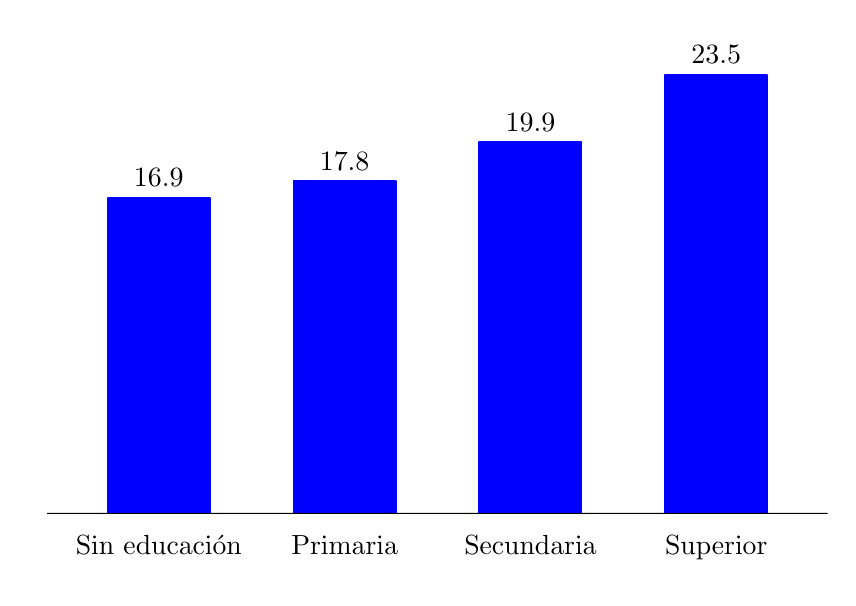
\begin{tikzpicture}[x=1pt,y=1pt]  % Created by tikzDevice version 0.7.0 on 2015-09-08 18:21:26
% !TEX encoding = UTF-8 Unicode
\definecolor[named]{fillColor}{rgb}{1.00,1.00,1.00}
\path[use as bounding box,fill=fillColor,fill opacity=0.00] (0,0) rectangle (289.08,198.74);
\begin{scope}
\path[clip] (  0.00,  0.00) rectangle (289.08,198.74);
\definecolor[named]{drawColor}{rgb}{1.00,1.00,1.00}

\path[draw=drawColor,line width= 0.6pt,line join=round,line cap=round] (  0.00,  0.00) rectangle (289.08,198.74);
\end{scope}
\begin{scope}
\path[clip] (  0.00,  0.00) rectangle (289.08,198.74);

\path[] (  7.11, 23.47) rectangle (289.08,181.67);

\path[] ( 47.39, 23.47) --
	( 47.39,181.67);

\path[] (114.53, 23.47) --
	(114.53,181.67);

\path[] (181.66, 23.47) --
	(181.66,181.67);

\path[] (248.80, 23.47) --
	(248.80,181.67);
\definecolor[named]{drawColor}{rgb}{0.00,0.00,1.00}
\definecolor[named]{fillColor}{rgb}{0.00,0.00,1.00}

\path[draw=drawColor,line width= 0.6pt,line join=round,fill=fillColor] ( 28.93, 23.47) rectangle ( 65.86,137.24);

\path[draw=drawColor,line width= 0.6pt,line join=round,fill=fillColor] ( 96.07, 23.47) rectangle (132.99,143.30);

\path[draw=drawColor,line width= 0.6pt,line join=round,fill=fillColor] (163.20, 23.47) rectangle (200.13,157.44);

\path[draw=drawColor,line width= 0.6pt,line join=round,fill=fillColor] (230.34, 23.47) rectangle (267.26,181.67);
\definecolor[named]{drawColor}{rgb}{0.00,0.00,0.00}
\definecolor[named]{fillColor}{rgb}{0.00,0.00,0.00}

\path[draw=drawColor,line width= 0.1pt,line join=round,fill=fillColor] (  7.11, 23.47) -- (289.08, 23.47);

\node[text=drawColor,anchor=base,inner sep=0pt, outer sep=0pt, scale=  1.01] at ( 47.39,141.20) {16.9};

\node[text=drawColor,anchor=base,inner sep=0pt, outer sep=0pt, scale=  1.01] at (114.53,147.25) {17.8};

\node[text=drawColor,anchor=base,inner sep=0pt, outer sep=0pt, scale=  1.01] at (181.66,161.39) {19.9};

\node[text=drawColor,anchor=base,inner sep=0pt, outer sep=0pt, scale=  1.01] at (248.80,185.63) {23.5};
\end{scope}
\begin{scope}
\path[clip] (  0.00,  0.00) rectangle (289.08,198.74);

\path[] (  7.11, 23.47) --
	(  7.11,181.67);
\end{scope}
\begin{scope}
\path[clip] (  0.00,  0.00) rectangle (289.08,198.74);

\path[] (  7.11, 23.47) --
	(289.08, 23.47);
\end{scope}
\begin{scope}
\path[clip] (  0.00,  0.00) rectangle (289.08,198.74);

\path[] ( 47.39, 19.20) --
	( 47.39, 23.47);

\path[] (114.53, 19.20) --
	(114.53, 23.47);

\path[] (181.66, 19.20) --
	(181.66, 23.47);

\path[] (248.80, 19.20) --
	(248.80, 23.47);
\end{scope}
\begin{scope}
\path[clip] (  0.00,  0.00) rectangle (289.08,198.74);
\definecolor[named]{drawColor}{rgb}{0.00,0.00,0.00}

\node[text=drawColor,anchor=base,inner sep=0pt, outer sep=0pt, scale=  1.00] at ( 47.39,  8.54) {Sin educaci\'on};

\node[text=drawColor,anchor=base,inner sep=0pt, outer sep=0pt, scale=  1.00] at (114.53,  8.54) {Primaria};

\node[text=drawColor,anchor=base,inner sep=0pt, outer sep=0pt, scale=  1.00] at (181.66,  8.54) {Secundaria};

\node[text=drawColor,anchor=base,inner sep=0pt, outer sep=0pt, scale=  1.00] at (248.80,  8.54) {Superior};
\end{scope}
  \end{tikzpicture}}{Instituto Nacional de Estadística, con datos de la Encuesta Nacional de Salud Materno Infantil}

%
%\cajita{Primera relación sexual de mujeres sin educación}{}{Edad mediana de la primera relación sexual de las mujeres sin ningún nivel educativo alcanzado}{República de Guatemala, serie histórica por ENSMI, años}{\ \\[0mm]\begin{tikzpicture}[x=1pt,y=1pt]  % Created by tikzDevice version 0.7.0 on 2015-08-28 14:52:23
% !TEX encoding = UTF-8 Unicode
\definecolor[named]{fillColor}{rgb}{1.00,1.00,1.00}
\path[use as bounding box,fill=fillColor,fill opacity=0.00] (0,0) rectangle (289.08,198.74);
\begin{scope}
\path[clip] (  0.00,  0.00) rectangle (289.08,198.74);
\definecolor[named]{drawColor}{rgb}{1.00,1.00,1.00}

\path[draw=drawColor,line width= 0.6pt,line join=round,line cap=round] (  0.00,  0.00) rectangle (289.08,198.74);
\end{scope}
\begin{scope}
\path[clip] (  0.00,  0.00) rectangle (289.08,198.74);

\path[] ( 19.57, 17.78) rectangle (280.54,191.48);

\path[] ( 19.57, 39.49) --
	(280.54, 39.49);

\path[] ( 19.57, 82.92) --
	(280.54, 82.92);

\path[] ( 19.57,126.34) --
	(280.54,126.34);

\path[] ( 19.57,169.77) --
	(280.54,169.77);

\path[] ( 19.57, 17.78) --
	(280.54, 17.78);

\path[] ( 19.57, 61.20) --
	(280.54, 61.20);

\path[] ( 19.57,104.63) --
	(280.54,104.63);

\path[] ( 19.57,148.06) --
	(280.54,148.06);

\path[] ( 19.57,191.48) --
	(280.54,191.48);

\path[] ( 49.69, 17.78) --
	( 49.69,191.48);

\path[] ( 99.87, 17.78) --
	( 99.87,191.48);

\path[] (150.06, 17.78) --
	(150.06,191.48);

\path[] (200.25, 17.78) --
	(200.25,191.48);

\path[] (250.43, 17.78) --
	(250.43,191.48);
\definecolor[named]{drawColor}{rgb}{0.00,0.00,1.00}

\path[draw=drawColor,line width= 1.7pt,line join=round] ( 49.69,104.63) --
	( 99.87,104.63) --
	(150.06,104.63) --
	(200.25,104.63) --
	(250.43,104.63);
\definecolor[named]{drawColor}{rgb}{0.00,0.00,0.00}

\node[text=drawColor,anchor=base,inner sep=0pt, outer sep=0pt, scale=  1.01] at ( 49.69,108.59) {0};

\node[text=drawColor,anchor=base,inner sep=0pt, outer sep=0pt, scale=  1.01] at ( 99.87,108.59) {0};

\node[text=drawColor,anchor=base,inner sep=0pt, outer sep=0pt, scale=  1.01] at (150.06,108.59) {0};

\node[text=drawColor,anchor=base,inner sep=0pt, outer sep=0pt, scale=  1.01] at (200.25,108.59) {0};

\node[text=drawColor,anchor=base,inner sep=0pt, outer sep=0pt, scale=  1.01] at (250.43,108.59) {0};
\definecolor[named]{fillColor}{rgb}{0.00,0.00,0.00}

\path[draw=drawColor,line width= 0.1pt,line join=round,fill=fillColor] ( 19.57,104.63) -- (280.54,104.63);
\end{scope}
\begin{scope}
\path[clip] (  0.00,  0.00) rectangle (289.08,198.74);

\path[] ( 19.57, 17.78) --
	( 19.57,191.48);
\end{scope}
\begin{scope}
\path[clip] (  0.00,  0.00) rectangle (289.08,198.74);
\definecolor[named]{drawColor}{rgb}{1.00,1.00,1.00}

\node[text=drawColor,text opacity=0.00,anchor=base east,inner sep=0pt, outer sep=0pt, scale=  1.00] at ( 12.46, 13.87) {-0.50};

\node[text=drawColor,text opacity=0.00,anchor=base east,inner sep=0pt, outer sep=0pt, scale=  1.00] at ( 12.46, 57.29) {-0.25};

\node[text=drawColor,text opacity=0.00,anchor=base east,inner sep=0pt, outer sep=0pt, scale=  1.00] at ( 12.46,100.72) {0.00};

\node[text=drawColor,text opacity=0.00,anchor=base east,inner sep=0pt, outer sep=0pt, scale=  1.00] at ( 12.46,144.15) {0.25};

\node[text=drawColor,text opacity=0.00,anchor=base east,inner sep=0pt, outer sep=0pt, scale=  1.00] at ( 12.46,187.57) {0.50};
\end{scope}
\begin{scope}
\path[clip] (  0.00,  0.00) rectangle (289.08,198.74);

\path[] ( 15.31, 17.78) --
	( 19.57, 17.78);

\path[] ( 15.31, 61.20) --
	( 19.57, 61.20);

\path[] ( 15.31,104.63) --
	( 19.57,104.63);

\path[] ( 15.31,148.06) --
	( 19.57,148.06);

\path[] ( 15.31,191.48) --
	( 19.57,191.48);
\end{scope}
\begin{scope}
\path[clip] (  0.00,  0.00) rectangle (289.08,198.74);

\path[] ( 19.57, 17.78) --
	(280.54, 17.78);
\end{scope}
\begin{scope}
\path[clip] (  0.00,  0.00) rectangle (289.08,198.74);

\path[] ( 49.69, 13.51) --
	( 49.69, 17.78);

\path[] ( 99.87, 13.51) --
	( 99.87, 17.78);

\path[] (150.06, 13.51) --
	(150.06, 17.78);

\path[] (200.25, 13.51) --
	(200.25, 17.78);

\path[] (250.43, 13.51) --
	(250.43, 17.78);
\end{scope}
\begin{scope}
\path[clip] (  0.00,  0.00) rectangle (289.08,198.74);
\definecolor[named]{drawColor}{rgb}{0.00,0.00,0.00}

\node[text=drawColor,anchor=base,inner sep=0pt, outer sep=0pt, scale=  1.00] at ( 49.69,  2.85) {1987};

\node[text=drawColor,anchor=base,inner sep=0pt, outer sep=0pt, scale=  1.00] at ( 99.87,  2.85) {1995};

\node[text=drawColor,anchor=base,inner sep=0pt, outer sep=0pt, scale=  1.00] at (150.06,  2.85) {1998/99};

\node[text=drawColor,anchor=base,inner sep=0pt, outer sep=0pt, scale=  1.00] at (200.25,  2.85) {2002};

\node[text=drawColor,anchor=base,inner sep=0pt, outer sep=0pt, scale=  1.00] at (250.43,  2.85) {2008/09};
\end{scope}
  \end{tikzpicture}}{Instituto Nacional de Estadística, con datos de la Encuesta Nacional de Salud Materno Infantil}


%
%\cajita{Primer nacimiento}{}{Edad mediana del primer nacimiento en mujeres entre 20 y 49 años}{República de Guatemala, serie histórica por ENSMI, años}{\ \\[0mm]\begin{tikzpicture}[x=1pt,y=1pt]  % Created by tikzDevice version 0.7.0 on 2015-08-28 14:52:23
% !TEX encoding = UTF-8 Unicode
\definecolor[named]{fillColor}{rgb}{1.00,1.00,1.00}
\path[use as bounding box,fill=fillColor,fill opacity=0.00] (0,0) rectangle (289.08,198.74);
\begin{scope}
\path[clip] (  0.00,  0.00) rectangle (289.08,198.74);
\definecolor[named]{drawColor}{rgb}{1.00,1.00,1.00}

\path[draw=drawColor,line width= 0.6pt,line join=round,line cap=round] (  0.00,  0.00) rectangle (289.08,198.74);
\end{scope}
\begin{scope}
\path[clip] (  0.00,  0.00) rectangle (289.08,198.74);

\path[] (  7.11, 20.62) rectangle (289.08,174.77);

\path[] ( 39.65, 20.62) --
	( 39.65,174.77);

\path[] ( 93.87, 20.62) --
	( 93.87,174.77);

\path[] (148.10, 20.62) --
	(148.10,174.77);

\path[] (202.32, 20.62) --
	(202.32,174.77);

\path[] (256.55, 20.62) --
	(256.55,174.77);
\definecolor[named]{drawColor}{rgb}{0.00,0.00,1.00}
\definecolor[named]{fillColor}{rgb}{0.00,0.00,1.00}

\path[draw=drawColor,line width= 0.6pt,line join=round,fill=fillColor] ( 18.64, 20.62) rectangle ( 36.26,174.77);
\definecolor[named]{drawColor}{rgb}{0.62,0.73,1.00}
\definecolor[named]{fillColor}{rgb}{0.62,0.73,1.00}

\path[draw=drawColor,line width= 0.6pt,line join=round,fill=fillColor] ( 43.04, 20.62) rectangle ( 60.66,155.50);
\definecolor[named]{drawColor}{rgb}{0.00,0.00,1.00}
\definecolor[named]{fillColor}{rgb}{0.00,0.00,1.00}

\path[draw=drawColor,line width= 0.6pt,line join=round,fill=fillColor] ( 72.86, 20.62) rectangle ( 90.48,161.00);
\definecolor[named]{drawColor}{rgb}{0.62,0.73,1.00}
\definecolor[named]{fillColor}{rgb}{0.62,0.73,1.00}

\path[draw=drawColor,line width= 0.6pt,line join=round,fill=fillColor] ( 97.26, 20.62) rectangle (114.88,130.72);
\definecolor[named]{drawColor}{rgb}{0.00,0.00,1.00}
\definecolor[named]{fillColor}{rgb}{0.00,0.00,1.00}

\path[draw=drawColor,line width= 0.6pt,line join=round,fill=fillColor] (127.08, 20.62) rectangle (144.71,158.25);
\definecolor[named]{drawColor}{rgb}{0.62,0.73,1.00}
\definecolor[named]{fillColor}{rgb}{0.62,0.73,1.00}

\path[draw=drawColor,line width= 0.6pt,line join=round,fill=fillColor] (151.49, 20.62) rectangle (169.11,133.48);
\definecolor[named]{drawColor}{rgb}{0.00,0.00,1.00}
\definecolor[named]{fillColor}{rgb}{0.00,0.00,1.00}

\path[draw=drawColor,line width= 0.6pt,line join=round,fill=fillColor] (181.31, 20.62) rectangle (198.93,141.73);
\definecolor[named]{drawColor}{rgb}{0.62,0.73,1.00}
\definecolor[named]{fillColor}{rgb}{0.62,0.73,1.00}

\path[draw=drawColor,line width= 0.6pt,line join=round,fill=fillColor] (205.71, 20.62) rectangle (223.33,122.47);
\definecolor[named]{drawColor}{rgb}{0.00,0.00,1.00}
\definecolor[named]{fillColor}{rgb}{0.00,0.00,1.00}

\path[draw=drawColor,line width= 0.6pt,line join=round,fill=fillColor] (235.53, 20.62) rectangle (253.16,119.71);
\definecolor[named]{drawColor}{rgb}{0.62,0.73,1.00}
\definecolor[named]{fillColor}{rgb}{0.62,0.73,1.00}

\path[draw=drawColor,line width= 0.6pt,line join=round,fill=fillColor] (259.93, 20.62) rectangle (277.56,100.45);
\definecolor[named]{drawColor}{rgb}{0.00,0.00,0.00}
\definecolor[named]{fillColor}{rgb}{0.00,0.00,0.00}

\path[draw=drawColor,line width= 0.6pt,line join=round,fill=fillColor] (  7.11, 20.62) -- (289.08, 20.62);

\node[text=drawColor,anchor=base,inner sep=0pt, outer sep=0pt, scale=  0.82] at ( 27.45,177.99) {5.6};

\node[text=drawColor,anchor=base,inner sep=0pt, outer sep=0pt, scale=  0.82] at ( 51.85,158.72) {4.9};

\node[text=drawColor,anchor=base,inner sep=0pt, outer sep=0pt, scale=  0.82] at ( 81.67,164.23) {5.1};

\node[text=drawColor,anchor=base,inner sep=0pt, outer sep=0pt, scale=  0.82] at (106.07,133.95) {4.0};

\node[text=drawColor,anchor=base,inner sep=0pt, outer sep=0pt, scale=  0.82] at (135.90,161.47) {5.0};

\node[text=drawColor,anchor=base,inner sep=0pt, outer sep=0pt, scale=  0.82] at (160.30,136.70) {4.1};

\node[text=drawColor,anchor=base,inner sep=0pt, outer sep=0pt, scale=  0.82] at (190.12,144.96) {4.4};

\node[text=drawColor,anchor=base,inner sep=0pt, outer sep=0pt, scale=  0.82] at (214.52,125.69) {3.7};

\node[text=drawColor,anchor=base,inner sep=0pt, outer sep=0pt, scale=  0.82] at (244.34,122.94) {3.6};

\node[text=drawColor,anchor=base,inner sep=0pt, outer sep=0pt, scale=  0.82] at (268.75,103.67) {2.9};
\end{scope}
\begin{scope}
\path[clip] (  0.00,  0.00) rectangle (289.08,198.74);

\path[] (  7.11, 20.62) --
	(  7.11,174.77);
\end{scope}
\begin{scope}
\path[clip] (  0.00,  0.00) rectangle (289.08,198.74);

\path[] (  7.11, 20.62) --
	(289.08, 20.62);
\end{scope}
\begin{scope}
\path[clip] (  0.00,  0.00) rectangle (289.08,198.74);

\path[] ( 39.65, 16.35) --
	( 39.65, 20.62);

\path[] ( 93.87, 16.35) --
	( 93.87, 20.62);

\path[] (148.10, 16.35) --
	(148.10, 20.62);

\path[] (202.32, 16.35) --
	(202.32, 20.62);

\path[] (256.55, 16.35) --
	(256.55, 20.62);
\end{scope}
\begin{scope}
\path[clip] (  0.00,  0.00) rectangle (289.08,198.74);
\definecolor[named]{drawColor}{rgb}{0.00,0.00,0.00}

\node[text=drawColor,anchor=base,inner sep=0pt, outer sep=0pt, scale=  1.00] at ( 39.65,  5.69) {1987};

\node[text=drawColor,anchor=base,inner sep=0pt, outer sep=0pt, scale=  1.00] at ( 93.87,  5.69) {1995};

\node[text=drawColor,anchor=base,inner sep=0pt, outer sep=0pt, scale=  1.00] at (148.10,  5.69) {1998/99};

\node[text=drawColor,anchor=base,inner sep=0pt, outer sep=0pt, scale=  1.00] at (202.32,  5.69) {2002};

\node[text=drawColor,anchor=base,inner sep=0pt, outer sep=0pt, scale=  1.00] at (256.55,  5.69) {2008/09};
\end{scope}
\coordinate (apoyo) at (50.29,191.13);
\coordinate (longitudFicticia) at (7.11,7.61);
\coordinate (longitud) at (7.11,7.11);
\coordinate (desX) at (142.09,0);
\coordinate (desY) at (0,0.25);
\definecolor[named]{ct1}{HTML}{
0000FF
}
\definecolor[named]{ct2}{HTML}{
9DBBFF
}
\definecolor[named]{ctb1}{HTML}{
0000FF
}
\definecolor[named]{ctb2}{HTML}{
9DBBFF
}
\path [fill=none] (apoyo) rectangle ($(apoyo)+(longitudFicticia)$)
node [xshift=0.3cm,inner sep=0pt, outer sep=0pt,midway,right,scale = 0.9]{Observados};
\draw [color = ctb1,fill=ct1] ( $(apoyo)  + (desY) $) rectangle ($(apoyo)+ (desY) +(longitud)$);
\path [fill=none] ($(apoyo)+(desX)$) rectangle ($(apoyo)+(desX)+(longitudFicticia)$)
node [xshift=0.3cm,inner sep=0pt, outer sep=0pt,midway,right,scale = 0.9]{Deseados};
\draw [color = ctb2 ,fill=ct2] ( $(apoyo)  + (desY) + (desX) $) rectangle ($(apoyo)+ (desY)+ (desX) +(longitud)$);
  \end{tikzpicture}}{Instituto Nacional de Estadística, con datos de la Encuesta Nacional de Salud Materno Infantil}
%
%
%\cajita{Primer nacimiento según escolaridad}{}{Edad mediana del primer nacimiento en mujeres entre 20 y 49 años, por nivel de educación}{República de Guatemala, 2008-09, años}{\ \\[0mm]\begin{tikzpicture}[x=1pt,y=1pt]  % Created by tikzDevice version 0.7.0 on 2015-09-01 14:20:56
% !TEX encoding = UTF-8 Unicode
\definecolor[named]{fillColor}{rgb}{1.00,1.00,1.00}
\path[use as bounding box,fill=fillColor,fill opacity=0.00] (0,0) rectangle (289.08,198.74);
\begin{scope}
\path[clip] (  0.00,  0.00) rectangle (289.08,198.74);
\definecolor[named]{drawColor}{rgb}{1.00,1.00,1.00}

\path[draw=drawColor,line width= 0.6pt,line join=round,line cap=round] (  0.00,  0.00) rectangle (289.08,198.74);
\end{scope}
\begin{scope}
\path[clip] (  0.00,  0.00) rectangle (289.08,198.74);

\path[] (  7.11, 20.62) rectangle (289.08,174.77);

\path[] ( 59.98, 20.62) --
	( 59.98,174.77);

\path[] (148.10, 20.62) --
	(148.10,174.77);

\path[] (236.21, 20.62) --
	(236.21,174.77);
\definecolor[named]{drawColor}{rgb}{0.00,0.00,1.00}
\definecolor[named]{fillColor}{rgb}{0.00,0.00,1.00}

\path[draw=drawColor,line width= 0.6pt,line join=round,fill=fillColor] ( 28.04, 20.62) rectangle ( 52.27,174.77);
\definecolor[named]{drawColor}{rgb}{0.62,0.73,1.00}
\definecolor[named]{fillColor}{rgb}{0.62,0.73,1.00}

\path[draw=drawColor,line width= 0.6pt,line join=round,fill=fillColor] ( 67.69, 20.62) rectangle ( 91.92,145.12);
\definecolor[named]{drawColor}{rgb}{0.00,0.00,1.00}
\definecolor[named]{fillColor}{rgb}{0.00,0.00,1.00}

\path[draw=drawColor,line width= 0.6pt,line join=round,fill=fillColor] (116.16, 20.62) rectangle (140.39,133.27);
\definecolor[named]{drawColor}{rgb}{0.62,0.73,1.00}
\definecolor[named]{fillColor}{rgb}{0.62,0.73,1.00}

\path[draw=drawColor,line width= 0.6pt,line join=round,fill=fillColor] (155.81, 20.62) rectangle (180.04,112.51);
\definecolor[named]{drawColor}{rgb}{0.00,0.00,1.00}
\definecolor[named]{fillColor}{rgb}{0.00,0.00,1.00}

\path[draw=drawColor,line width= 0.6pt,line join=round,fill=fillColor] (204.27, 20.62) rectangle (228.50, 88.80);
\definecolor[named]{drawColor}{rgb}{0.62,0.73,1.00}
\definecolor[named]{fillColor}{rgb}{0.62,0.73,1.00}

\path[draw=drawColor,line width= 0.6pt,line join=round,fill=fillColor] (243.92, 20.62) rectangle (268.15, 76.94);
\definecolor[named]{drawColor}{rgb}{0.00,0.00,0.00}
\definecolor[named]{fillColor}{rgb}{0.00,0.00,0.00}

\path[draw=drawColor,line width= 0.6pt,line join=round,fill=fillColor] (  7.11, 20.62) -- (289.08, 20.62);

\node[text=drawColor,anchor=base,inner sep=0pt, outer sep=0pt, scale=  0.82] at ( 40.16,177.99) {5.2};

\node[text=drawColor,anchor=base,inner sep=0pt, outer sep=0pt, scale=  0.82] at ( 79.81,148.35) {4.2};

\node[text=drawColor,anchor=base,inner sep=0pt, outer sep=0pt, scale=  0.82] at (128.27,136.49) {3.8};

\node[text=drawColor,anchor=base,inner sep=0pt, outer sep=0pt, scale=  0.82] at (167.92,115.74) {3.1};

\node[text=drawColor,anchor=base,inner sep=0pt, outer sep=0pt, scale=  0.82] at (216.39, 92.02) {2.3};

\node[text=drawColor,anchor=base,inner sep=0pt, outer sep=0pt, scale=  0.82] at (256.04, 80.17) {1.9};
\end{scope}
\begin{scope}
\path[clip] (  0.00,  0.00) rectangle (289.08,198.74);

\path[] (  7.11, 20.62) --
	(  7.11,174.77);
\end{scope}
\begin{scope}
\path[clip] (  0.00,  0.00) rectangle (289.08,198.74);

\path[] (  7.11, 20.62) --
	(289.08, 20.62);
\end{scope}
\begin{scope}
\path[clip] (  0.00,  0.00) rectangle (289.08,198.74);

\path[] ( 59.98, 16.35) --
	( 59.98, 20.62);

\path[] (148.10, 16.35) --
	(148.10, 20.62);

\path[] (236.21, 16.35) --
	(236.21, 20.62);
\end{scope}
\begin{scope}
\path[clip] (  0.00,  0.00) rectangle (289.08,198.74);
\definecolor[named]{drawColor}{rgb}{0.00,0.00,0.00}

\node[text=drawColor,anchor=base,inner sep=0pt, outer sep=0pt, scale=  1.00] at ( 59.98,  5.69) {Sin educaci\'on};

\node[text=drawColor,anchor=base,inner sep=0pt, outer sep=0pt, scale=  1.00] at (148.10,  5.69) {Primaria};

\node[text=drawColor,anchor=base,inner sep=0pt, outer sep=0pt, scale=  1.00] at (236.21,  5.69) {Secundaria o superior};
\end{scope}
\coordinate (apoyo) at (50.29,191.13);
\coordinate (longitudFicticia) at (7.11,7.61);
\coordinate (longitud) at (7.11,7.11);
\coordinate (desX) at (142.09,0);
\coordinate (desY) at (0,0.25);
\definecolor[named]{ct1}{HTML}{
0000FF
}
\definecolor[named]{ct2}{HTML}{
9DBBFF
}
\definecolor[named]{ctb1}{HTML}{
0000FF
}
\definecolor[named]{ctb2}{HTML}{
9DBBFF
}
\path [fill=none] (apoyo) rectangle ($(apoyo)+(longitudFicticia)$)
node [xshift=0.3cm,inner sep=0pt, outer sep=0pt,midway,right,scale = 0.9]{Observados};
\draw [color = ctb1,fill=ct1] ( $(apoyo)  + (desY) $) rectangle ($(apoyo)+ (desY) +(longitud)$);
\path [fill=none] ($(apoyo)+(desX)$) rectangle ($(apoyo)+(desX)+(longitudFicticia)$)
node [xshift=0.3cm,inner sep=0pt, outer sep=0pt,midway,right,scale = 0.9]{Deseados};
\draw [color = ctb2 ,fill=ct2] ( $(apoyo)  + (desY) + (desX) $) rectangle ($(apoyo)+ (desY)+ (desX) +(longitud)$);
  \end{tikzpicture}}{Instituto Nacional de Estadística, con datos de la Encuesta Nacional de Salud Materno Infantil}
%
%
%\cajita{Primer nacimiento, mujeres sin educación}{}{Edad mediana del primer nacimiento en mujeres sin educación, entre 20 y 49 años}{República de Guatemala, serie histórica por ENSMI, años}{\ \\[0mm]\begin{tikzpicture}[x=1pt,y=1pt]  % Created by tikzDevice version 0.7.0 on 2015-08-28 14:52:30
% !TEX encoding = UTF-8 Unicode
\definecolor[named]{fillColor}{rgb}{1.00,1.00,1.00}
\path[use as bounding box,fill=fillColor,fill opacity=0.00] (0,0) rectangle (289.08,198.74);
\begin{scope}
\path[clip] (  0.00,  0.00) rectangle (289.08,198.74);
\definecolor[named]{drawColor}{rgb}{1.00,1.00,1.00}

\path[draw=drawColor,line width= 0.6pt,line join=round,line cap=round] (  0.00,  0.00) rectangle (289.08,198.74);
\end{scope}
\begin{scope}
\path[clip] (  0.00,  0.00) rectangle (289.08,198.74);

\path[] (  7.11, 20.62) rectangle (289.08,174.77);

\path[] ( 39.65, 20.62) --
	( 39.65,174.77);

\path[] ( 93.87, 20.62) --
	( 93.87,174.77);

\path[] (148.10, 20.62) --
	(148.10,174.77);

\path[] (202.32, 20.62) --
	(202.32,174.77);

\path[] (256.55, 20.62) --
	(256.55,174.77);
\definecolor[named]{drawColor}{rgb}{0.00,0.00,1.00}
\definecolor[named]{fillColor}{rgb}{0.00,0.00,1.00}

\path[draw=drawColor,line width= 0.6pt,line join=round,fill=fillColor] ( 18.64, 20.62) rectangle ( 36.26,172.59);
\definecolor[named]{drawColor}{rgb}{0.62,0.73,1.00}
\definecolor[named]{fillColor}{rgb}{0.62,0.73,1.00}

\path[draw=drawColor,line width= 0.6pt,line join=round,fill=fillColor] ( 43.04, 20.62) rectangle ( 60.66,155.23);
\definecolor[named]{drawColor}{rgb}{0.00,0.00,1.00}
\definecolor[named]{fillColor}{rgb}{0.00,0.00,1.00}

\path[draw=drawColor,line width= 0.6pt,line join=round,fill=fillColor] ( 72.86, 20.62) rectangle ( 90.48,174.77);
\definecolor[named]{drawColor}{rgb}{0.62,0.73,1.00}
\definecolor[named]{fillColor}{rgb}{0.62,0.73,1.00}

\path[draw=drawColor,line width= 0.6pt,line join=round,fill=fillColor] ( 97.26, 20.62) rectangle (114.88,142.20);
\definecolor[named]{drawColor}{rgb}{0.00,0.00,1.00}
\definecolor[named]{fillColor}{rgb}{0.00,0.00,1.00}

\path[draw=drawColor,line width= 0.6pt,line join=round,fill=fillColor] (127.08, 20.62) rectangle (144.71,168.25);
\definecolor[named]{drawColor}{rgb}{0.62,0.73,1.00}
\definecolor[named]{fillColor}{rgb}{0.62,0.73,1.00}

\path[draw=drawColor,line width= 0.6pt,line join=round,fill=fillColor] (151.49, 20.62) rectangle (169.11,144.37);
\definecolor[named]{drawColor}{rgb}{0.00,0.00,1.00}
\definecolor[named]{fillColor}{rgb}{0.00,0.00,1.00}

\path[draw=drawColor,line width= 0.6pt,line join=round,fill=fillColor] (181.31, 20.62) rectangle (198.93,159.57);
\definecolor[named]{drawColor}{rgb}{0.62,0.73,1.00}
\definecolor[named]{fillColor}{rgb}{0.62,0.73,1.00}

\path[draw=drawColor,line width= 0.6pt,line join=round,fill=fillColor] (205.71, 20.62) rectangle (223.33,135.69);
\definecolor[named]{drawColor}{rgb}{0.00,0.00,1.00}
\definecolor[named]{fillColor}{rgb}{0.00,0.00,1.00}

\path[draw=drawColor,line width= 0.6pt,line join=round,fill=fillColor] (235.53, 20.62) rectangle (253.16,133.52);
\definecolor[named]{drawColor}{rgb}{0.62,0.73,1.00}
\definecolor[named]{fillColor}{rgb}{0.62,0.73,1.00}

\path[draw=drawColor,line width= 0.6pt,line join=round,fill=fillColor] (259.93, 20.62) rectangle (277.56,111.81);
\definecolor[named]{drawColor}{rgb}{0.00,0.00,0.00}
\definecolor[named]{fillColor}{rgb}{0.00,0.00,0.00}

\path[draw=drawColor,line width= 0.6pt,line join=round,fill=fillColor] (  7.11, 20.62) -- (289.08, 20.62);

\node[text=drawColor,anchor=base,inner sep=0pt, outer sep=0pt, scale=  0.82] at ( 27.45,175.82) {7.0};

\node[text=drawColor,anchor=base,inner sep=0pt, outer sep=0pt, scale=  0.82] at ( 51.85,158.45) {6.2};

\node[text=drawColor,anchor=base,inner sep=0pt, outer sep=0pt, scale=  0.82] at ( 81.67,177.99) {7.1};

\node[text=drawColor,anchor=base,inner sep=0pt, outer sep=0pt, scale=  0.82] at (106.07,145.42) {5.6};

\node[text=drawColor,anchor=base,inner sep=0pt, outer sep=0pt, scale=  0.82] at (135.90,171.48) {6.8};

\node[text=drawColor,anchor=base,inner sep=0pt, outer sep=0pt, scale=  0.82] at (160.30,147.59) {5.7};

\node[text=drawColor,anchor=base,inner sep=0pt, outer sep=0pt, scale=  0.82] at (190.12,162.79) {6.4};

\node[text=drawColor,anchor=base,inner sep=0pt, outer sep=0pt, scale=  0.82] at (214.52,138.91) {5.3};

\node[text=drawColor,anchor=base,inner sep=0pt, outer sep=0pt, scale=  0.82] at (244.34,136.74) {5.2};

\node[text=drawColor,anchor=base,inner sep=0pt, outer sep=0pt, scale=  0.82] at (268.75,115.03) {4.2};
\end{scope}
\begin{scope}
\path[clip] (  0.00,  0.00) rectangle (289.08,198.74);

\path[] (  7.11, 20.62) --
	(  7.11,174.77);
\end{scope}
\begin{scope}
\path[clip] (  0.00,  0.00) rectangle (289.08,198.74);

\path[] (  7.11, 20.62) --
	(289.08, 20.62);
\end{scope}
\begin{scope}
\path[clip] (  0.00,  0.00) rectangle (289.08,198.74);

\path[] ( 39.65, 16.35) --
	( 39.65, 20.62);

\path[] ( 93.87, 16.35) --
	( 93.87, 20.62);

\path[] (148.10, 16.35) --
	(148.10, 20.62);

\path[] (202.32, 16.35) --
	(202.32, 20.62);

\path[] (256.55, 16.35) --
	(256.55, 20.62);
\end{scope}
\begin{scope}
\path[clip] (  0.00,  0.00) rectangle (289.08,198.74);
\definecolor[named]{drawColor}{rgb}{0.00,0.00,0.00}

\node[text=drawColor,anchor=base,inner sep=0pt, outer sep=0pt, scale=  1.00] at ( 39.65,  5.69) {1987};

\node[text=drawColor,anchor=base,inner sep=0pt, outer sep=0pt, scale=  1.00] at ( 93.87,  5.69) {1995};

\node[text=drawColor,anchor=base,inner sep=0pt, outer sep=0pt, scale=  1.00] at (148.10,  5.69) {1998/99};

\node[text=drawColor,anchor=base,inner sep=0pt, outer sep=0pt, scale=  1.00] at (202.32,  5.69) {2002};

\node[text=drawColor,anchor=base,inner sep=0pt, outer sep=0pt, scale=  1.00] at (256.55,  5.69) {2008/09};
\end{scope}
\coordinate (apoyo) at (50.29,191.13);
\coordinate (longitudFicticia) at (7.11,7.61);
\coordinate (longitud) at (7.11,7.11);
\coordinate (desX) at (142.09,0);
\coordinate (desY) at (0,0.25);
\definecolor[named]{ct1}{HTML}{
0000FF
}
\definecolor[named]{ct2}{HTML}{
9DBBFF
}
\definecolor[named]{ctb1}{HTML}{
0000FF
}
\definecolor[named]{ctb2}{HTML}{
9DBBFF
}
\path [fill=none] (apoyo) rectangle ($(apoyo)+(longitudFicticia)$)
node [xshift=0.3cm,inner sep=0pt, outer sep=0pt,midway,right,scale = 0.9]{Observados};
\draw [color = ctb1,fill=ct1] ( $(apoyo)  + (desY) $) rectangle ($(apoyo)+ (desY) +(longitud)$);
\path [fill=none] ($(apoyo)+(desX)$) rectangle ($(apoyo)+(desX)+(longitudFicticia)$)
node [xshift=0.3cm,inner sep=0pt, outer sep=0pt,midway,right,scale = 0.9]{Deseados};
\draw [color = ctb2 ,fill=ct2] ( $(apoyo)  + (desY) + (desX) $) rectangle ($(apoyo)+ (desY)+ (desX) +(longitud)$);
  \end{tikzpicture}}{Instituto Nacional de Estadística, con datos de la Encuesta Nacional de Salud Materno Infantil}

%


\cajita{Cantidad de hijos deseados y observados}{
	La tasa de fecundidad deseada y observada, según los datos reportados en las encuestas nacionales de salud materno infantil, muestra que,  en general,  la tasa observada es mayor en un hijo, respecto a lo deseado.
	}{Tasa de fecundidad deseada y observada}{República de Guatemala, serie histórica por ENSMI, niños por mujer}{\ \\[0mm]\begin{tikzpicture}[x=1pt,y=1pt]  % Created by tikzDevice version 0.7.0 on 2015-08-28 14:52:23
% !TEX encoding = UTF-8 Unicode
\definecolor[named]{fillColor}{rgb}{1.00,1.00,1.00}
\path[use as bounding box,fill=fillColor,fill opacity=0.00] (0,0) rectangle (289.08,198.74);
\begin{scope}
\path[clip] (  0.00,  0.00) rectangle (289.08,198.74);
\definecolor[named]{drawColor}{rgb}{1.00,1.00,1.00}

\path[draw=drawColor,line width= 0.6pt,line join=round,line cap=round] (  0.00,  0.00) rectangle (289.08,198.74);
\end{scope}
\begin{scope}
\path[clip] (  0.00,  0.00) rectangle (289.08,198.74);

\path[] (  7.11, 20.62) rectangle (289.08,174.77);

\path[] ( 39.65, 20.62) --
	( 39.65,174.77);

\path[] ( 93.87, 20.62) --
	( 93.87,174.77);

\path[] (148.10, 20.62) --
	(148.10,174.77);

\path[] (202.32, 20.62) --
	(202.32,174.77);

\path[] (256.55, 20.62) --
	(256.55,174.77);
\definecolor[named]{drawColor}{rgb}{0.00,0.00,1.00}
\definecolor[named]{fillColor}{rgb}{0.00,0.00,1.00}

\path[draw=drawColor,line width= 0.6pt,line join=round,fill=fillColor] ( 18.64, 20.62) rectangle ( 36.26,174.77);
\definecolor[named]{drawColor}{rgb}{0.62,0.73,1.00}
\definecolor[named]{fillColor}{rgb}{0.62,0.73,1.00}

\path[draw=drawColor,line width= 0.6pt,line join=round,fill=fillColor] ( 43.04, 20.62) rectangle ( 60.66,155.50);
\definecolor[named]{drawColor}{rgb}{0.00,0.00,1.00}
\definecolor[named]{fillColor}{rgb}{0.00,0.00,1.00}

\path[draw=drawColor,line width= 0.6pt,line join=round,fill=fillColor] ( 72.86, 20.62) rectangle ( 90.48,161.00);
\definecolor[named]{drawColor}{rgb}{0.62,0.73,1.00}
\definecolor[named]{fillColor}{rgb}{0.62,0.73,1.00}

\path[draw=drawColor,line width= 0.6pt,line join=round,fill=fillColor] ( 97.26, 20.62) rectangle (114.88,130.72);
\definecolor[named]{drawColor}{rgb}{0.00,0.00,1.00}
\definecolor[named]{fillColor}{rgb}{0.00,0.00,1.00}

\path[draw=drawColor,line width= 0.6pt,line join=round,fill=fillColor] (127.08, 20.62) rectangle (144.71,158.25);
\definecolor[named]{drawColor}{rgb}{0.62,0.73,1.00}
\definecolor[named]{fillColor}{rgb}{0.62,0.73,1.00}

\path[draw=drawColor,line width= 0.6pt,line join=round,fill=fillColor] (151.49, 20.62) rectangle (169.11,133.48);
\definecolor[named]{drawColor}{rgb}{0.00,0.00,1.00}
\definecolor[named]{fillColor}{rgb}{0.00,0.00,1.00}

\path[draw=drawColor,line width= 0.6pt,line join=round,fill=fillColor] (181.31, 20.62) rectangle (198.93,141.73);
\definecolor[named]{drawColor}{rgb}{0.62,0.73,1.00}
\definecolor[named]{fillColor}{rgb}{0.62,0.73,1.00}

\path[draw=drawColor,line width= 0.6pt,line join=round,fill=fillColor] (205.71, 20.62) rectangle (223.33,122.47);
\definecolor[named]{drawColor}{rgb}{0.00,0.00,1.00}
\definecolor[named]{fillColor}{rgb}{0.00,0.00,1.00}

\path[draw=drawColor,line width= 0.6pt,line join=round,fill=fillColor] (235.53, 20.62) rectangle (253.16,119.71);
\definecolor[named]{drawColor}{rgb}{0.62,0.73,1.00}
\definecolor[named]{fillColor}{rgb}{0.62,0.73,1.00}

\path[draw=drawColor,line width= 0.6pt,line join=round,fill=fillColor] (259.93, 20.62) rectangle (277.56,100.45);
\definecolor[named]{drawColor}{rgb}{0.00,0.00,0.00}
\definecolor[named]{fillColor}{rgb}{0.00,0.00,0.00}

\path[draw=drawColor,line width= 0.6pt,line join=round,fill=fillColor] (  7.11, 20.62) -- (289.08, 20.62);

\node[text=drawColor,anchor=base,inner sep=0pt, outer sep=0pt, scale=  0.82] at ( 27.45,177.99) {5.6};

\node[text=drawColor,anchor=base,inner sep=0pt, outer sep=0pt, scale=  0.82] at ( 51.85,158.72) {4.9};

\node[text=drawColor,anchor=base,inner sep=0pt, outer sep=0pt, scale=  0.82] at ( 81.67,164.23) {5.1};

\node[text=drawColor,anchor=base,inner sep=0pt, outer sep=0pt, scale=  0.82] at (106.07,133.95) {4.0};

\node[text=drawColor,anchor=base,inner sep=0pt, outer sep=0pt, scale=  0.82] at (135.90,161.47) {5.0};

\node[text=drawColor,anchor=base,inner sep=0pt, outer sep=0pt, scale=  0.82] at (160.30,136.70) {4.1};

\node[text=drawColor,anchor=base,inner sep=0pt, outer sep=0pt, scale=  0.82] at (190.12,144.96) {4.4};

\node[text=drawColor,anchor=base,inner sep=0pt, outer sep=0pt, scale=  0.82] at (214.52,125.69) {3.7};

\node[text=drawColor,anchor=base,inner sep=0pt, outer sep=0pt, scale=  0.82] at (244.34,122.94) {3.6};

\node[text=drawColor,anchor=base,inner sep=0pt, outer sep=0pt, scale=  0.82] at (268.75,103.67) {2.9};
\end{scope}
\begin{scope}
\path[clip] (  0.00,  0.00) rectangle (289.08,198.74);

\path[] (  7.11, 20.62) --
	(  7.11,174.77);
\end{scope}
\begin{scope}
\path[clip] (  0.00,  0.00) rectangle (289.08,198.74);

\path[] (  7.11, 20.62) --
	(289.08, 20.62);
\end{scope}
\begin{scope}
\path[clip] (  0.00,  0.00) rectangle (289.08,198.74);

\path[] ( 39.65, 16.35) --
	( 39.65, 20.62);

\path[] ( 93.87, 16.35) --
	( 93.87, 20.62);

\path[] (148.10, 16.35) --
	(148.10, 20.62);

\path[] (202.32, 16.35) --
	(202.32, 20.62);

\path[] (256.55, 16.35) --
	(256.55, 20.62);
\end{scope}
\begin{scope}
\path[clip] (  0.00,  0.00) rectangle (289.08,198.74);
\definecolor[named]{drawColor}{rgb}{0.00,0.00,0.00}

\node[text=drawColor,anchor=base,inner sep=0pt, outer sep=0pt, scale=  1.00] at ( 39.65,  5.69) {1987};

\node[text=drawColor,anchor=base,inner sep=0pt, outer sep=0pt, scale=  1.00] at ( 93.87,  5.69) {1995};

\node[text=drawColor,anchor=base,inner sep=0pt, outer sep=0pt, scale=  1.00] at (148.10,  5.69) {1998/99};

\node[text=drawColor,anchor=base,inner sep=0pt, outer sep=0pt, scale=  1.00] at (202.32,  5.69) {2002};

\node[text=drawColor,anchor=base,inner sep=0pt, outer sep=0pt, scale=  1.00] at (256.55,  5.69) {2008/09};
\end{scope}
\coordinate (apoyo) at (50.29,191.13);
\coordinate (longitudFicticia) at (7.11,7.61);
\coordinate (longitud) at (7.11,7.11);
\coordinate (desX) at (142.09,0);
\coordinate (desY) at (0,0.25);
\definecolor[named]{ct1}{HTML}{
0000FF
}
\definecolor[named]{ct2}{HTML}{
9DBBFF
}
\definecolor[named]{ctb1}{HTML}{
0000FF
}
\definecolor[named]{ctb2}{HTML}{
9DBBFF
}
\path [fill=none] (apoyo) rectangle ($(apoyo)+(longitudFicticia)$)
node [xshift=0.3cm,inner sep=0pt, outer sep=0pt,midway,right,scale = 0.9]{Observados};
\draw [color = ctb1,fill=ct1] ( $(apoyo)  + (desY) $) rectangle ($(apoyo)+ (desY) +(longitud)$);
\path [fill=none] ($(apoyo)+(desX)$) rectangle ($(apoyo)+(desX)+(longitudFicticia)$)
node [xshift=0.3cm,inner sep=0pt, outer sep=0pt,midway,right,scale = 0.9]{Deseados};
\draw [color = ctb2 ,fill=ct2] ( $(apoyo)  + (desY) + (desX) $) rectangle ($(apoyo)+ (desY)+ (desX) +(longitud)$);
  \end{tikzpicture}}{Instituto Nacional de Estadística, con datos de la Encuesta Nacional de Salud Materno Infantil}


\cajita{Cantidad de hijos deseados y observados según escolaridad}{Según el grado de escolaridad de las mujeres, la tasa de fecundidad deseada en aquellas con educación superior es de 1.9 hijos y la observada de 2.3 hijos por mujer.\\
	
	La tasa más alta se presenta en mujeres sin educación, con una tasa deseada de hijos de 4.2 mientras que la observada en este grupo es de 5.2 hijos por mujer.}{Tasa de fecundidad deseada y observada por nivel de educación}{República de Guatemala, 2008-09, niños por mujer}{\ \\[0mm]\begin{tikzpicture}[x=1pt,y=1pt]  % Created by tikzDevice version 0.7.0 on 2015-09-01 14:20:56
% !TEX encoding = UTF-8 Unicode
\definecolor[named]{fillColor}{rgb}{1.00,1.00,1.00}
\path[use as bounding box,fill=fillColor,fill opacity=0.00] (0,0) rectangle (289.08,198.74);
\begin{scope}
\path[clip] (  0.00,  0.00) rectangle (289.08,198.74);
\definecolor[named]{drawColor}{rgb}{1.00,1.00,1.00}

\path[draw=drawColor,line width= 0.6pt,line join=round,line cap=round] (  0.00,  0.00) rectangle (289.08,198.74);
\end{scope}
\begin{scope}
\path[clip] (  0.00,  0.00) rectangle (289.08,198.74);

\path[] (  7.11, 20.62) rectangle (289.08,174.77);

\path[] ( 59.98, 20.62) --
	( 59.98,174.77);

\path[] (148.10, 20.62) --
	(148.10,174.77);

\path[] (236.21, 20.62) --
	(236.21,174.77);
\definecolor[named]{drawColor}{rgb}{0.00,0.00,1.00}
\definecolor[named]{fillColor}{rgb}{0.00,0.00,1.00}

\path[draw=drawColor,line width= 0.6pt,line join=round,fill=fillColor] ( 28.04, 20.62) rectangle ( 52.27,174.77);
\definecolor[named]{drawColor}{rgb}{0.62,0.73,1.00}
\definecolor[named]{fillColor}{rgb}{0.62,0.73,1.00}

\path[draw=drawColor,line width= 0.6pt,line join=round,fill=fillColor] ( 67.69, 20.62) rectangle ( 91.92,145.12);
\definecolor[named]{drawColor}{rgb}{0.00,0.00,1.00}
\definecolor[named]{fillColor}{rgb}{0.00,0.00,1.00}

\path[draw=drawColor,line width= 0.6pt,line join=round,fill=fillColor] (116.16, 20.62) rectangle (140.39,133.27);
\definecolor[named]{drawColor}{rgb}{0.62,0.73,1.00}
\definecolor[named]{fillColor}{rgb}{0.62,0.73,1.00}

\path[draw=drawColor,line width= 0.6pt,line join=round,fill=fillColor] (155.81, 20.62) rectangle (180.04,112.51);
\definecolor[named]{drawColor}{rgb}{0.00,0.00,1.00}
\definecolor[named]{fillColor}{rgb}{0.00,0.00,1.00}

\path[draw=drawColor,line width= 0.6pt,line join=round,fill=fillColor] (204.27, 20.62) rectangle (228.50, 88.80);
\definecolor[named]{drawColor}{rgb}{0.62,0.73,1.00}
\definecolor[named]{fillColor}{rgb}{0.62,0.73,1.00}

\path[draw=drawColor,line width= 0.6pt,line join=round,fill=fillColor] (243.92, 20.62) rectangle (268.15, 76.94);
\definecolor[named]{drawColor}{rgb}{0.00,0.00,0.00}
\definecolor[named]{fillColor}{rgb}{0.00,0.00,0.00}

\path[draw=drawColor,line width= 0.6pt,line join=round,fill=fillColor] (  7.11, 20.62) -- (289.08, 20.62);

\node[text=drawColor,anchor=base,inner sep=0pt, outer sep=0pt, scale=  0.82] at ( 40.16,177.99) {5.2};

\node[text=drawColor,anchor=base,inner sep=0pt, outer sep=0pt, scale=  0.82] at ( 79.81,148.35) {4.2};

\node[text=drawColor,anchor=base,inner sep=0pt, outer sep=0pt, scale=  0.82] at (128.27,136.49) {3.8};

\node[text=drawColor,anchor=base,inner sep=0pt, outer sep=0pt, scale=  0.82] at (167.92,115.74) {3.1};

\node[text=drawColor,anchor=base,inner sep=0pt, outer sep=0pt, scale=  0.82] at (216.39, 92.02) {2.3};

\node[text=drawColor,anchor=base,inner sep=0pt, outer sep=0pt, scale=  0.82] at (256.04, 80.17) {1.9};
\end{scope}
\begin{scope}
\path[clip] (  0.00,  0.00) rectangle (289.08,198.74);

\path[] (  7.11, 20.62) --
	(  7.11,174.77);
\end{scope}
\begin{scope}
\path[clip] (  0.00,  0.00) rectangle (289.08,198.74);

\path[] (  7.11, 20.62) --
	(289.08, 20.62);
\end{scope}
\begin{scope}
\path[clip] (  0.00,  0.00) rectangle (289.08,198.74);

\path[] ( 59.98, 16.35) --
	( 59.98, 20.62);

\path[] (148.10, 16.35) --
	(148.10, 20.62);

\path[] (236.21, 16.35) --
	(236.21, 20.62);
\end{scope}
\begin{scope}
\path[clip] (  0.00,  0.00) rectangle (289.08,198.74);
\definecolor[named]{drawColor}{rgb}{0.00,0.00,0.00}

\node[text=drawColor,anchor=base,inner sep=0pt, outer sep=0pt, scale=  1.00] at ( 59.98,  5.69) {Sin educaci\'on};

\node[text=drawColor,anchor=base,inner sep=0pt, outer sep=0pt, scale=  1.00] at (148.10,  5.69) {Primaria};

\node[text=drawColor,anchor=base,inner sep=0pt, outer sep=0pt, scale=  1.00] at (236.21,  5.69) {Secundaria o superior};
\end{scope}
\coordinate (apoyo) at (50.29,191.13);
\coordinate (longitudFicticia) at (7.11,7.61);
\coordinate (longitud) at (7.11,7.11);
\coordinate (desX) at (142.09,0);
\coordinate (desY) at (0,0.25);
\definecolor[named]{ct1}{HTML}{
0000FF
}
\definecolor[named]{ct2}{HTML}{
9DBBFF
}
\definecolor[named]{ctb1}{HTML}{
0000FF
}
\definecolor[named]{ctb2}{HTML}{
9DBBFF
}
\path [fill=none] (apoyo) rectangle ($(apoyo)+(longitudFicticia)$)
node [xshift=0.3cm,inner sep=0pt, outer sep=0pt,midway,right,scale = 0.9]{Observados};
\draw [color = ctb1,fill=ct1] ( $(apoyo)  + (desY) $) rectangle ($(apoyo)+ (desY) +(longitud)$);
\path [fill=none] ($(apoyo)+(desX)$) rectangle ($(apoyo)+(desX)+(longitudFicticia)$)
node [xshift=0.3cm,inner sep=0pt, outer sep=0pt,midway,right,scale = 0.9]{Deseados};
\draw [color = ctb2 ,fill=ct2] ( $(apoyo)  + (desY) + (desX) $) rectangle ($(apoyo)+ (desY)+ (desX) +(longitud)$);
  \end{tikzpicture}}{Instituto Nacional de Estadística, con datos de la Encuesta Nacional de Salud Materno Infantil}


\cajita{Cantidad de hijos deseados y observados en mujeres sin educación}{La tasa de hijos deseados en mujeres sin educación tiene una tendencia descendente, de 6.2 hijos por mujer en la encuesta realizada en 1987 a 4.2 en el 2008-09. Esto es una disminución de 2 hijos por mujer.}{Tasa de fecundidad deseada y observada en mujeres sin ningún nivel educativo alcanzado}{República de Guatemala, serie histórica por ENSMI, niños por mujer}{\ \\[0mm]\begin{tikzpicture}[x=1pt,y=1pt]  % Created by tikzDevice version 0.7.0 on 2015-08-28 14:52:30
% !TEX encoding = UTF-8 Unicode
\definecolor[named]{fillColor}{rgb}{1.00,1.00,1.00}
\path[use as bounding box,fill=fillColor,fill opacity=0.00] (0,0) rectangle (289.08,198.74);
\begin{scope}
\path[clip] (  0.00,  0.00) rectangle (289.08,198.74);
\definecolor[named]{drawColor}{rgb}{1.00,1.00,1.00}

\path[draw=drawColor,line width= 0.6pt,line join=round,line cap=round] (  0.00,  0.00) rectangle (289.08,198.74);
\end{scope}
\begin{scope}
\path[clip] (  0.00,  0.00) rectangle (289.08,198.74);

\path[] (  7.11, 20.62) rectangle (289.08,174.77);

\path[] ( 39.65, 20.62) --
	( 39.65,174.77);

\path[] ( 93.87, 20.62) --
	( 93.87,174.77);

\path[] (148.10, 20.62) --
	(148.10,174.77);

\path[] (202.32, 20.62) --
	(202.32,174.77);

\path[] (256.55, 20.62) --
	(256.55,174.77);
\definecolor[named]{drawColor}{rgb}{0.00,0.00,1.00}
\definecolor[named]{fillColor}{rgb}{0.00,0.00,1.00}

\path[draw=drawColor,line width= 0.6pt,line join=round,fill=fillColor] ( 18.64, 20.62) rectangle ( 36.26,172.59);
\definecolor[named]{drawColor}{rgb}{0.62,0.73,1.00}
\definecolor[named]{fillColor}{rgb}{0.62,0.73,1.00}

\path[draw=drawColor,line width= 0.6pt,line join=round,fill=fillColor] ( 43.04, 20.62) rectangle ( 60.66,155.23);
\definecolor[named]{drawColor}{rgb}{0.00,0.00,1.00}
\definecolor[named]{fillColor}{rgb}{0.00,0.00,1.00}

\path[draw=drawColor,line width= 0.6pt,line join=round,fill=fillColor] ( 72.86, 20.62) rectangle ( 90.48,174.77);
\definecolor[named]{drawColor}{rgb}{0.62,0.73,1.00}
\definecolor[named]{fillColor}{rgb}{0.62,0.73,1.00}

\path[draw=drawColor,line width= 0.6pt,line join=round,fill=fillColor] ( 97.26, 20.62) rectangle (114.88,142.20);
\definecolor[named]{drawColor}{rgb}{0.00,0.00,1.00}
\definecolor[named]{fillColor}{rgb}{0.00,0.00,1.00}

\path[draw=drawColor,line width= 0.6pt,line join=round,fill=fillColor] (127.08, 20.62) rectangle (144.71,168.25);
\definecolor[named]{drawColor}{rgb}{0.62,0.73,1.00}
\definecolor[named]{fillColor}{rgb}{0.62,0.73,1.00}

\path[draw=drawColor,line width= 0.6pt,line join=round,fill=fillColor] (151.49, 20.62) rectangle (169.11,144.37);
\definecolor[named]{drawColor}{rgb}{0.00,0.00,1.00}
\definecolor[named]{fillColor}{rgb}{0.00,0.00,1.00}

\path[draw=drawColor,line width= 0.6pt,line join=round,fill=fillColor] (181.31, 20.62) rectangle (198.93,159.57);
\definecolor[named]{drawColor}{rgb}{0.62,0.73,1.00}
\definecolor[named]{fillColor}{rgb}{0.62,0.73,1.00}

\path[draw=drawColor,line width= 0.6pt,line join=round,fill=fillColor] (205.71, 20.62) rectangle (223.33,135.69);
\definecolor[named]{drawColor}{rgb}{0.00,0.00,1.00}
\definecolor[named]{fillColor}{rgb}{0.00,0.00,1.00}

\path[draw=drawColor,line width= 0.6pt,line join=round,fill=fillColor] (235.53, 20.62) rectangle (253.16,133.52);
\definecolor[named]{drawColor}{rgb}{0.62,0.73,1.00}
\definecolor[named]{fillColor}{rgb}{0.62,0.73,1.00}

\path[draw=drawColor,line width= 0.6pt,line join=round,fill=fillColor] (259.93, 20.62) rectangle (277.56,111.81);
\definecolor[named]{drawColor}{rgb}{0.00,0.00,0.00}
\definecolor[named]{fillColor}{rgb}{0.00,0.00,0.00}

\path[draw=drawColor,line width= 0.6pt,line join=round,fill=fillColor] (  7.11, 20.62) -- (289.08, 20.62);

\node[text=drawColor,anchor=base,inner sep=0pt, outer sep=0pt, scale=  0.82] at ( 27.45,175.82) {7.0};

\node[text=drawColor,anchor=base,inner sep=0pt, outer sep=0pt, scale=  0.82] at ( 51.85,158.45) {6.2};

\node[text=drawColor,anchor=base,inner sep=0pt, outer sep=0pt, scale=  0.82] at ( 81.67,177.99) {7.1};

\node[text=drawColor,anchor=base,inner sep=0pt, outer sep=0pt, scale=  0.82] at (106.07,145.42) {5.6};

\node[text=drawColor,anchor=base,inner sep=0pt, outer sep=0pt, scale=  0.82] at (135.90,171.48) {6.8};

\node[text=drawColor,anchor=base,inner sep=0pt, outer sep=0pt, scale=  0.82] at (160.30,147.59) {5.7};

\node[text=drawColor,anchor=base,inner sep=0pt, outer sep=0pt, scale=  0.82] at (190.12,162.79) {6.4};

\node[text=drawColor,anchor=base,inner sep=0pt, outer sep=0pt, scale=  0.82] at (214.52,138.91) {5.3};

\node[text=drawColor,anchor=base,inner sep=0pt, outer sep=0pt, scale=  0.82] at (244.34,136.74) {5.2};

\node[text=drawColor,anchor=base,inner sep=0pt, outer sep=0pt, scale=  0.82] at (268.75,115.03) {4.2};
\end{scope}
\begin{scope}
\path[clip] (  0.00,  0.00) rectangle (289.08,198.74);

\path[] (  7.11, 20.62) --
	(  7.11,174.77);
\end{scope}
\begin{scope}
\path[clip] (  0.00,  0.00) rectangle (289.08,198.74);

\path[] (  7.11, 20.62) --
	(289.08, 20.62);
\end{scope}
\begin{scope}
\path[clip] (  0.00,  0.00) rectangle (289.08,198.74);

\path[] ( 39.65, 16.35) --
	( 39.65, 20.62);

\path[] ( 93.87, 16.35) --
	( 93.87, 20.62);

\path[] (148.10, 16.35) --
	(148.10, 20.62);

\path[] (202.32, 16.35) --
	(202.32, 20.62);

\path[] (256.55, 16.35) --
	(256.55, 20.62);
\end{scope}
\begin{scope}
\path[clip] (  0.00,  0.00) rectangle (289.08,198.74);
\definecolor[named]{drawColor}{rgb}{0.00,0.00,0.00}

\node[text=drawColor,anchor=base,inner sep=0pt, outer sep=0pt, scale=  1.00] at ( 39.65,  5.69) {1987};

\node[text=drawColor,anchor=base,inner sep=0pt, outer sep=0pt, scale=  1.00] at ( 93.87,  5.69) {1995};

\node[text=drawColor,anchor=base,inner sep=0pt, outer sep=0pt, scale=  1.00] at (148.10,  5.69) {1998/99};

\node[text=drawColor,anchor=base,inner sep=0pt, outer sep=0pt, scale=  1.00] at (202.32,  5.69) {2002};

\node[text=drawColor,anchor=base,inner sep=0pt, outer sep=0pt, scale=  1.00] at (256.55,  5.69) {2008/09};
\end{scope}
\coordinate (apoyo) at (50.29,191.13);
\coordinate (longitudFicticia) at (7.11,7.61);
\coordinate (longitud) at (7.11,7.11);
\coordinate (desX) at (142.09,0);
\coordinate (desY) at (0,0.25);
\definecolor[named]{ct1}{HTML}{
0000FF
}
\definecolor[named]{ct2}{HTML}{
9DBBFF
}
\definecolor[named]{ctb1}{HTML}{
0000FF
}
\definecolor[named]{ctb2}{HTML}{
9DBBFF
}
\path [fill=none] (apoyo) rectangle ($(apoyo)+(longitudFicticia)$)
node [xshift=0.3cm,inner sep=0pt, outer sep=0pt,midway,right,scale = 0.9]{Observados};
\draw [color = ctb1,fill=ct1] ( $(apoyo)  + (desY) $) rectangle ($(apoyo)+ (desY) +(longitud)$);
\path [fill=none] ($(apoyo)+(desX)$) rectangle ($(apoyo)+(desX)+(longitudFicticia)$)
node [xshift=0.3cm,inner sep=0pt, outer sep=0pt,midway,right,scale = 0.9]{Deseados};
\draw [color = ctb2 ,fill=ct2] ( $(apoyo)  + (desY) + (desX) $) rectangle ($(apoyo)+ (desY)+ (desX) +(longitud)$);
  \end{tikzpicture}}{Instituto Nacional de Estadística, con datos de la Encuesta Nacional de Salud Materno Infantil}

%

\cajita{Conocimiento de métodos anticonceptivos}{De las mujeres que viven en unión, la tendencia sobre el conocimiento en el uso de métodos de planificación familiar ha ido en crecimiento, de 71.9\% (1987)  a  97.4\% (2008-09).}{Proporción de mujeres en unión que conocen algún método de planificación familiar}{República de Guatemala, serie histórica por ENSMI, en porcentaje}{\ \\[0mm]\begin{tikzpicture}[x=1pt,y=1pt]  % Created by tikzDevice version 0.7.0 on 2015-09-01 14:23:11
% !TEX encoding = UTF-8 Unicode
\definecolor[named]{fillColor}{rgb}{1.00,1.00,1.00}
\path[use as bounding box,fill=fillColor,fill opacity=0.00] (0,0) rectangle (289.08,198.74);
\begin{scope}
\path[clip] (  0.00,  0.00) rectangle (289.08,198.74);
\definecolor[named]{drawColor}{rgb}{1.00,1.00,1.00}

\path[draw=drawColor,line width= 0.6pt,line join=round,line cap=round] (  0.00,  0.00) rectangle (289.08,198.74);
\end{scope}
\begin{scope}
\path[clip] (  0.00,  0.00) rectangle (289.08,198.74);

\path[] (  6.02, 17.78) rectangle (280.54,191.48);

\path[] (  6.02, 25.67) --
	(280.54, 25.67);

\path[] (  6.02, 72.53) --
	(280.54, 72.53);

\path[] (  6.02,119.39) --
	(280.54,119.39);

\path[] (  6.02,166.25) --
	(280.54,166.25);

\path[] (  6.02, 49.10) --
	(280.54, 49.10);

\path[] (  6.02, 95.96) --
	(280.54, 95.96);

\path[] (  6.02,142.82) --
	(280.54,142.82);

\path[] (  6.02,189.68) --
	(280.54,189.68);

\path[] ( 37.70, 17.78) --
	( 37.70,191.48);

\path[] ( 90.49, 17.78) --
	( 90.49,191.48);

\path[] (143.28, 17.78) --
	(143.28,191.48);

\path[] (196.08, 17.78) --
	(196.08,191.48);

\path[] (248.87, 17.78) --
	(248.87,191.48);
\definecolor[named]{drawColor}{rgb}{0.00,0.00,1.00}

\path[draw=drawColor,line width= 1.7pt,line join=round] ( 37.70,123.84) --
	( 90.49,147.04) --
	(143.28,154.77) --
	(196.08,173.98) --
	(248.87,183.59);
\definecolor[named]{drawColor}{rgb}{0.00,0.00,0.00}

\node[text=drawColor,anchor=base,inner sep=0pt, outer sep=0pt, scale=  1.01] at ( 37.70,111.97) {71.9};

\node[text=drawColor,anchor=base east,inner sep=0pt, outer sep=0pt, scale=  1.01] at ( 87.37,147.04) {81.8};

\node[text=drawColor,anchor=base east,inner sep=0pt, outer sep=0pt, scale=  1.01] at (140.17,154.77) {85.1};

\node[text=drawColor,anchor=base east,inner sep=0pt, outer sep=0pt, scale=  1.01] at (192.96,173.98) {93.3};

\node[text=drawColor,anchor=base,inner sep=0pt, outer sep=0pt, scale=  1.01] at (248.87,187.54) {97.4};
\definecolor[named]{fillColor}{rgb}{0.00,0.00,0.00}

\path[draw=drawColor,line width= 0.1pt,line join=round,fill=fillColor] (  6.02, 25.67) -- (280.54, 25.67);
\end{scope}
\begin{scope}
\path[clip] (  0.00,  0.00) rectangle (289.08,198.74);

\path[] (  6.02, 17.78) --
	(  6.02,191.48);
\end{scope}
\begin{scope}
\path[clip] (  0.00,  0.00) rectangle (289.08,198.74);

\path[] (  1.76, 49.10) --
	(  6.02, 49.10);

\path[] (  1.76, 95.96) --
	(  6.02, 95.96);

\path[] (  1.76,142.82) --
	(  6.02,142.82);

\path[] (  1.76,189.68) --
	(  6.02,189.68);
\end{scope}
\begin{scope}
\path[clip] (  0.00,  0.00) rectangle (289.08,198.74);

\path[] (  6.02, 17.78) --
	(280.54, 17.78);
\end{scope}
\begin{scope}
\path[clip] (  0.00,  0.00) rectangle (289.08,198.74);

\path[] ( 37.70, 13.51) --
	( 37.70, 17.78);

\path[] ( 90.49, 13.51) --
	( 90.49, 17.78);

\path[] (143.28, 13.51) --
	(143.28, 17.78);

\path[] (196.08, 13.51) --
	(196.08, 17.78);

\path[] (248.87, 13.51) --
	(248.87, 17.78);
\end{scope}
\begin{scope}
\path[clip] (  0.00,  0.00) rectangle (289.08,198.74);
\definecolor[named]{drawColor}{rgb}{0.00,0.00,0.00}

\node[text=drawColor,anchor=base,inner sep=0pt, outer sep=0pt, scale=  1.00] at ( 37.70,  2.85) {1987};

\node[text=drawColor,anchor=base,inner sep=0pt, outer sep=0pt, scale=  1.00] at ( 90.49,  2.85) {1995};

\node[text=drawColor,anchor=base,inner sep=0pt, outer sep=0pt, scale=  1.00] at (143.28,  2.85) {1998/99};

\node[text=drawColor,anchor=base,inner sep=0pt, outer sep=0pt, scale=  1.00] at (196.08,  2.85) {2002};

\node[text=drawColor,anchor=base,inner sep=0pt, outer sep=0pt, scale=  1.00] at (248.87,  2.85) {2008/09};
\end{scope}
  \end{tikzpicture}}{Instituto Nacional de Estadística, con datos de la Encuesta Nacional de Salud Materno Infantil}


\cajita{Conocimiento de métodos anticonceptivos según escolaridad}{Según el nivel de escolaridad, el 100\% de las mujeres en unión con educación superior conoce acerca de métodos de planificación familiar.\\
	
	 El menor porcentaje se presenta en las mujeres en unión sin educación, con el 93.3\%.}{Proporción de mujeres en unión que conocen algún método de planificación familiar, por nivel de educación}{República de Guatemala, 2008-09, en porcentaje}{\ \\[0mm]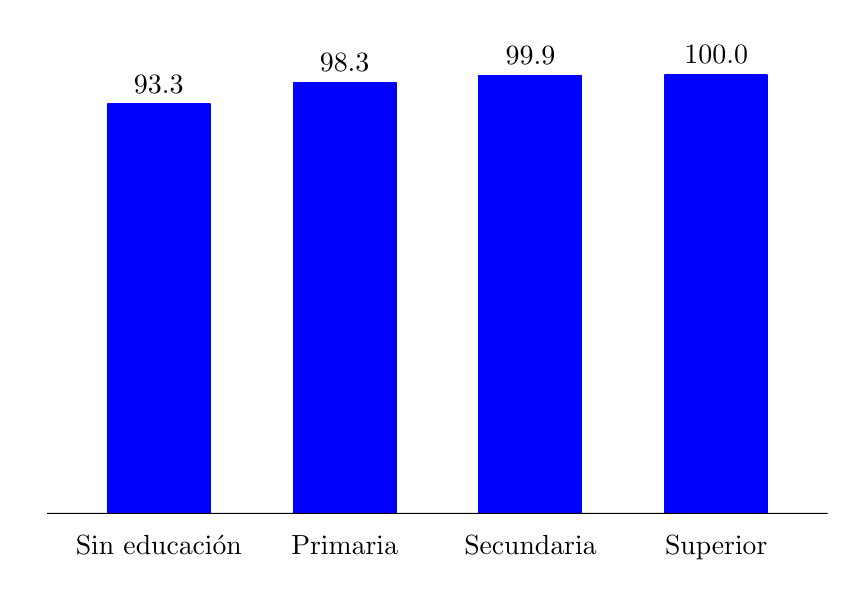
\begin{tikzpicture}[x=1pt,y=1pt]  % Created by tikzDevice version 0.7.0 on 2015-09-08 18:21:46
% !TEX encoding = UTF-8 Unicode
\definecolor[named]{fillColor}{rgb}{1.00,1.00,1.00}
\path[use as bounding box,fill=fillColor,fill opacity=0.00] (0,0) rectangle (289.08,198.74);
\begin{scope}
\path[clip] (  0.00,  0.00) rectangle (289.08,198.74);
\definecolor[named]{drawColor}{rgb}{1.00,1.00,1.00}

\path[draw=drawColor,line width= 0.6pt,line join=round,line cap=round] (  0.00,  0.00) rectangle (289.08,198.74);
\end{scope}
\begin{scope}
\path[clip] (  0.00,  0.00) rectangle (289.08,198.74);

\path[] (  7.11, 23.47) rectangle (289.08,181.67);

\path[] ( 47.39, 23.47) --
	( 47.39,181.67);

\path[] (114.53, 23.47) --
	(114.53,181.67);

\path[] (181.66, 23.47) --
	(181.66,181.67);

\path[] (248.80, 23.47) --
	(248.80,181.67);
\definecolor[named]{drawColor}{rgb}{0.00,0.00,1.00}
\definecolor[named]{fillColor}{rgb}{0.00,0.00,1.00}

\path[draw=drawColor,line width= 0.6pt,line join=round,fill=fillColor] ( 28.93, 23.47) rectangle ( 65.86,171.07);

\path[draw=drawColor,line width= 0.6pt,line join=round,fill=fillColor] ( 96.07, 23.47) rectangle (132.99,178.98);

\path[draw=drawColor,line width= 0.6pt,line join=round,fill=fillColor] (163.20, 23.47) rectangle (200.13,181.51);

\path[draw=drawColor,line width= 0.6pt,line join=round,fill=fillColor] (230.34, 23.47) rectangle (267.26,181.67);
\definecolor[named]{drawColor}{rgb}{0.00,0.00,0.00}
\definecolor[named]{fillColor}{rgb}{0.00,0.00,0.00}

\path[draw=drawColor,line width= 0.1pt,line join=round,fill=fillColor] (  7.11, 23.47) -- (289.08, 23.47);

\node[text=drawColor,anchor=base,inner sep=0pt, outer sep=0pt, scale=  1.01] at ( 47.39,175.03) {93.3};

\node[text=drawColor,anchor=base,inner sep=0pt, outer sep=0pt, scale=  1.01] at (114.53,182.94) {98.3};

\node[text=drawColor,anchor=base,inner sep=0pt, outer sep=0pt, scale=  1.01] at (181.66,185.47) {99.9};

\node[text=drawColor,anchor=base,inner sep=0pt, outer sep=0pt, scale=  1.01] at (248.80,185.63) {100.0};
\end{scope}
\begin{scope}
\path[clip] (  0.00,  0.00) rectangle (289.08,198.74);

\path[] (  7.11, 23.47) --
	(  7.11,181.67);
\end{scope}
\begin{scope}
\path[clip] (  0.00,  0.00) rectangle (289.08,198.74);

\path[] (  7.11, 23.47) --
	(289.08, 23.47);
\end{scope}
\begin{scope}
\path[clip] (  0.00,  0.00) rectangle (289.08,198.74);

\path[] ( 47.39, 19.20) --
	( 47.39, 23.47);

\path[] (114.53, 19.20) --
	(114.53, 23.47);

\path[] (181.66, 19.20) --
	(181.66, 23.47);

\path[] (248.80, 19.20) --
	(248.80, 23.47);
\end{scope}
\begin{scope}
\path[clip] (  0.00,  0.00) rectangle (289.08,198.74);
\definecolor[named]{drawColor}{rgb}{0.00,0.00,0.00}

\node[text=drawColor,anchor=base,inner sep=0pt, outer sep=0pt, scale=  1.00] at ( 47.39,  8.54) {Sin educaci\'on};

\node[text=drawColor,anchor=base,inner sep=0pt, outer sep=0pt, scale=  1.00] at (114.53,  8.54) {Primaria};

\node[text=drawColor,anchor=base,inner sep=0pt, outer sep=0pt, scale=  1.00] at (181.66,  8.54) {Secundaria};

\node[text=drawColor,anchor=base,inner sep=0pt, outer sep=0pt, scale=  1.00] at (248.80,  8.54) {Superior};
\end{scope}
  \end{tikzpicture}}{Instituto Nacional de Estadística, con datos de la Encuesta Nacional de Salud Materno Infantil}


\cajita{Conocimiento de métodos anticonceptivos mujeres sin educación}{Las mujeres que viven en unión y que no tienen educación que tienen algún tipo de conocimiento sobre métodos de planificación familiar ha ido en aumento, del 53\% en 1987 al 93.3\% en el 2009.}{Proporción de mujeres en unión y sin educación, que conocen algún método de planificación familiar}{República de Guatemala, serie histórica por ENSMI, en porcentaje}{\ \\[0mm]\begin{tikzpicture}[x=1pt,y=1pt]  % Created by tikzDevice version 0.7.0 on 2015-09-01 14:24:00
% !TEX encoding = UTF-8 Unicode
\definecolor[named]{fillColor}{rgb}{1.00,1.00,1.00}
\path[use as bounding box,fill=fillColor,fill opacity=0.00] (0,0) rectangle (289.08,198.74);
\begin{scope}
\path[clip] (  0.00,  0.00) rectangle (289.08,198.74);
\definecolor[named]{drawColor}{rgb}{1.00,1.00,1.00}

\path[draw=drawColor,line width= 0.6pt,line join=round,line cap=round] (  0.00,  0.00) rectangle (289.08,198.74);
\end{scope}
\begin{scope}
\path[clip] (  0.00,  0.00) rectangle (289.08,198.74);

\path[] (  1.64, 17.78) rectangle (280.54,191.48);

\path[] (  1.64, 47.21) --
	(280.54, 47.21);

\path[] (  1.64, 90.30) --
	(280.54, 90.30);

\path[] (  1.64,133.39) --
	(280.54,133.39);

\path[] (  1.64,176.48) --
	(280.54,176.48);

\path[] (  1.64, 25.67) --
	(280.54, 25.67);

\path[] (  1.64, 68.76) --
	(280.54, 68.76);

\path[] (  1.64,111.85) --
	(280.54,111.85);

\path[] (  1.64,154.93) --
	(280.54,154.93);

\path[] ( 33.83, 17.78) --
	( 33.83,191.48);

\path[] ( 87.46, 17.78) --
	( 87.46,191.48);

\path[] (141.09, 17.78) --
	(141.09,191.48);

\path[] (194.73, 17.78) --
	(194.73,191.48);

\path[] (248.36, 17.78) --
	(248.36,191.48);
\definecolor[named]{drawColor}{rgb}{0.00,0.00,1.00}

\path[draw=drawColor,line width= 1.7pt,line join=round] ( 33.83, 96.77) --
	( 87.46,123.48) --
	(141.09,133.39) --
	(194.73,167.64) --
	(248.36,183.59);
\definecolor[named]{drawColor}{rgb}{0.00,0.00,0.00}

\node[text=drawColor,anchor=base,inner sep=0pt, outer sep=0pt, scale=  1.01] at ( 33.83, 84.90) {53.0};

\node[text=drawColor,anchor=base east,inner sep=0pt, outer sep=0pt, scale=  1.01] at ( 84.34,123.48) {65.4};

\node[text=drawColor,anchor=base east,inner sep=0pt, outer sep=0pt, scale=  1.01] at (137.98,133.39) {70.0};

\node[text=drawColor,anchor=base east,inner sep=0pt, outer sep=0pt, scale=  1.01] at (191.61,167.64) {85.9};

\node[text=drawColor,anchor=base,inner sep=0pt, outer sep=0pt, scale=  1.01] at (248.36,187.54) {93.3};
\definecolor[named]{fillColor}{rgb}{0.00,0.00,0.00}

\path[draw=drawColor,line width= 0.1pt,line join=round,fill=fillColor] (  1.64, 25.67) -- (280.54, 25.67);
\end{scope}
\begin{scope}
\path[clip] (  0.00,  0.00) rectangle (289.08,198.74);

\path[] (  1.64, 17.78) --
	(  1.64,191.48);
\end{scope}
\begin{scope}
\path[clip] (  0.00,  0.00) rectangle (289.08,198.74);

\path[] (  0.00, 25.67) --
	(  1.64, 25.67);

\path[] (  0.00, 68.76) --
	(  1.64, 68.76);

\path[] (  0.00,111.85) --
	(  1.64,111.85);

\path[] (  0.00,154.93) --
	(  1.64,154.93);
\end{scope}
\begin{scope}
\path[clip] (  0.00,  0.00) rectangle (289.08,198.74);

\path[] (  1.64, 17.78) --
	(280.54, 17.78);
\end{scope}
\begin{scope}
\path[clip] (  0.00,  0.00) rectangle (289.08,198.74);

\path[] ( 33.83, 13.51) --
	( 33.83, 17.78);

\path[] ( 87.46, 13.51) --
	( 87.46, 17.78);

\path[] (141.09, 13.51) --
	(141.09, 17.78);

\path[] (194.73, 13.51) --
	(194.73, 17.78);

\path[] (248.36, 13.51) --
	(248.36, 17.78);
\end{scope}
\begin{scope}
\path[clip] (  0.00,  0.00) rectangle (289.08,198.74);
\definecolor[named]{drawColor}{rgb}{0.00,0.00,0.00}

\node[text=drawColor,anchor=base,inner sep=0pt, outer sep=0pt, scale=  1.00] at ( 33.83,  2.85) {1987};

\node[text=drawColor,anchor=base,inner sep=0pt, outer sep=0pt, scale=  1.00] at ( 87.46,  2.85) {1995};

\node[text=drawColor,anchor=base,inner sep=0pt, outer sep=0pt, scale=  1.00] at (141.09,  2.85) {1998/99};

\node[text=drawColor,anchor=base,inner sep=0pt, outer sep=0pt, scale=  1.00] at (194.73,  2.85) {2002};

\node[text=drawColor,anchor=base,inner sep=0pt, outer sep=0pt, scale=  1.00] at (248.36,  2.85) {2008/09};
\end{scope}
  \end{tikzpicture}}{Instituto Nacional de Estadística, con datos de la Encuesta Nacional de Salud Materno Infantil}



\cajita{Uso de métodos anticonceptivos}{De las mujeres que viven en unión, la tendencia en  el uso de métodos de planificación familiar ha ido en crecimiento, de 23.2\% (1987)  a  54.1\% (2008-09).}{Proporción de mujeres en unión que usan algún método de planificación familiar}{República de Guatemala, serie histórica por ENSMI, en porcentaje}{\ \\[0mm]\begin{tikzpicture}[x=1pt,y=1pt]  % Created by tikzDevice version 0.7.0 on 2015-09-01 14:24:37
% !TEX encoding = UTF-8 Unicode
\definecolor[named]{fillColor}{rgb}{1.00,1.00,1.00}
\path[use as bounding box,fill=fillColor,fill opacity=0.00] (0,0) rectangle (289.08,198.74);
\begin{scope}
\path[clip] (  0.00,  0.00) rectangle (289.08,198.74);
\definecolor[named]{drawColor}{rgb}{1.00,1.00,1.00}

\path[draw=drawColor,line width= 0.6pt,line join=round,line cap=round] (  0.00,  0.00) rectangle (289.08,198.74);
\end{scope}
\begin{scope}
\path[clip] (  0.00,  0.00) rectangle (289.08,198.74);

\path[] (  1.64, 17.78) rectangle (280.54,191.48);

\path[] (  1.64, 54.86) --
	(280.54, 54.86);

\path[] (  1.64,113.24) --
	(280.54,113.24);

\path[] (  1.64,171.62) --
	(280.54,171.62);

\path[] (  1.64, 25.67) --
	(280.54, 25.67);

\path[] (  1.64, 84.05) --
	(280.54, 84.05);

\path[] (  1.64,142.43) --
	(280.54,142.43);

\path[] ( 33.83, 17.78) --
	( 33.83,191.48);

\path[] ( 87.46, 17.78) --
	( 87.46,191.48);

\path[] (141.09, 17.78) --
	(141.09,191.48);

\path[] (194.73, 17.78) --
	(194.73,191.48);

\path[] (248.36, 17.78) --
	(248.36,191.48);
\definecolor[named]{drawColor}{rgb}{0.00,0.00,1.00}

\path[draw=drawColor,line width= 1.7pt,line join=round] ( 33.83, 93.39) --
	( 87.46,117.33) --
	(141.09,137.18) --
	(194.73,152.06) --
	(248.36,183.59);
\definecolor[named]{drawColor}{rgb}{0.00,0.00,0.00}

\node[text=drawColor,anchor=base,inner sep=0pt, outer sep=0pt, scale=  1.01] at ( 33.83, 81.52) {23.2};

\node[text=drawColor,anchor=base east,inner sep=0pt, outer sep=0pt, scale=  1.01] at ( 84.34,117.33) {31.4};

\node[text=drawColor,anchor=base east,inner sep=0pt, outer sep=0pt, scale=  1.01] at (137.98,137.18) {38.2};

\node[text=drawColor,anchor=base east,inner sep=0pt, outer sep=0pt, scale=  1.01] at (191.61,152.06) {43.3};

\node[text=drawColor,anchor=base,inner sep=0pt, outer sep=0pt, scale=  1.01] at (248.36,187.54) {54.1};
\definecolor[named]{fillColor}{rgb}{0.00,0.00,0.00}

\path[draw=drawColor,line width= 0.1pt,line join=round,fill=fillColor] (  1.64, 25.67) -- (280.54, 25.67);
\end{scope}
\begin{scope}
\path[clip] (  0.00,  0.00) rectangle (289.08,198.74);

\path[] (  1.64, 17.78) --
	(  1.64,191.48);
\end{scope}
\begin{scope}
\path[clip] (  0.00,  0.00) rectangle (289.08,198.74);

\path[] (  0.00, 25.67) --
	(  1.64, 25.67);

\path[] (  0.00, 84.05) --
	(  1.64, 84.05);

\path[] (  0.00,142.43) --
	(  1.64,142.43);
\end{scope}
\begin{scope}
\path[clip] (  0.00,  0.00) rectangle (289.08,198.74);

\path[] (  1.64, 17.78) --
	(280.54, 17.78);
\end{scope}
\begin{scope}
\path[clip] (  0.00,  0.00) rectangle (289.08,198.74);

\path[] ( 33.83, 13.51) --
	( 33.83, 17.78);

\path[] ( 87.46, 13.51) --
	( 87.46, 17.78);

\path[] (141.09, 13.51) --
	(141.09, 17.78);

\path[] (194.73, 13.51) --
	(194.73, 17.78);

\path[] (248.36, 13.51) --
	(248.36, 17.78);
\end{scope}
\begin{scope}
\path[clip] (  0.00,  0.00) rectangle (289.08,198.74);
\definecolor[named]{drawColor}{rgb}{0.00,0.00,0.00}

\node[text=drawColor,anchor=base,inner sep=0pt, outer sep=0pt, scale=  1.00] at ( 33.83,  2.85) {1987};

\node[text=drawColor,anchor=base,inner sep=0pt, outer sep=0pt, scale=  1.00] at ( 87.46,  2.85) {1995};

\node[text=drawColor,anchor=base,inner sep=0pt, outer sep=0pt, scale=  1.00] at (141.09,  2.85) {1998/99};

\node[text=drawColor,anchor=base,inner sep=0pt, outer sep=0pt, scale=  1.00] at (194.73,  2.85) {2002};

\node[text=drawColor,anchor=base,inner sep=0pt, outer sep=0pt, scale=  1.00] at (248.36,  2.85) {2008/09};
\end{scope}
  \end{tikzpicture}}{Instituto Nacional de Estadística, con datos de la Encuesta Nacional de Salud Materno Infantil}


\cajita{Uso de métodos anticonceptivos según escolaridad}{Según el nivel de escolaridad, el 70.2\% de las mujeres en unión con educación superior usa algún método de planificación familiar.\\
	
	 El menor porcentaje se presenta en las mujeres en unión sin educación, con el 29.9\%.}{Proporción de mujeres en unión que usan algún método de planificación familiar, por nivel de educación}{República de Guatemala, 2008-09, en porcentaje}{\ \\[0mm]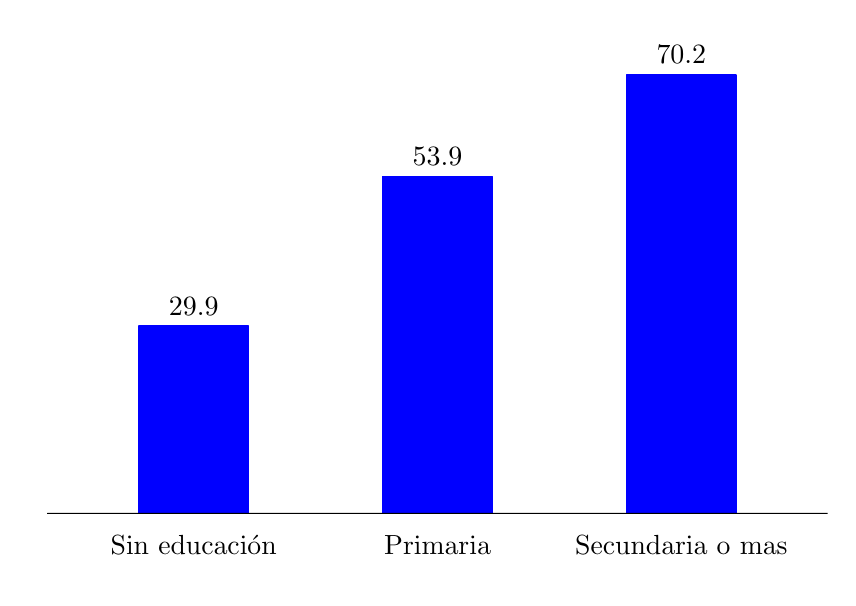
\begin{tikzpicture}[x=1pt,y=1pt]  % Created by tikzDevice version 0.7.0 on 2015-09-08 18:43:17
% !TEX encoding = UTF-8 Unicode
\definecolor[named]{fillColor}{rgb}{1.00,1.00,1.00}
\path[use as bounding box,fill=fillColor,fill opacity=0.00] (0,0) rectangle (289.08,198.74);
\begin{scope}
\path[clip] (  0.00,  0.00) rectangle (289.08,198.74);
\definecolor[named]{drawColor}{rgb}{1.00,1.00,1.00}

\path[draw=drawColor,line width= 0.6pt,line join=round,line cap=round] (  0.00,  0.00) rectangle (289.08,198.74);
\end{scope}
\begin{scope}
\path[clip] (  0.00,  0.00) rectangle (289.08,198.74);

\path[] (  7.11, 23.47) rectangle (289.08,181.67);

\path[] ( 59.98, 23.47) --
	( 59.98,181.67);

\path[] (148.10, 23.47) --
	(148.10,181.67);

\path[] (236.21, 23.47) --
	(236.21,181.67);
\definecolor[named]{drawColor}{rgb}{0.00,0.00,1.00}
\definecolor[named]{fillColor}{rgb}{0.00,0.00,1.00}

\path[draw=drawColor,line width= 0.6pt,line join=round,fill=fillColor] ( 40.16, 23.47) rectangle ( 79.81, 90.85);

\path[draw=drawColor,line width= 0.6pt,line join=round,fill=fillColor] (128.27, 23.47) rectangle (167.92,144.94);

\path[draw=drawColor,line width= 0.6pt,line join=round,fill=fillColor] (216.39, 23.47) rectangle (256.04,181.67);
\definecolor[named]{drawColor}{rgb}{0.00,0.00,0.00}
\definecolor[named]{fillColor}{rgb}{0.00,0.00,0.00}

\path[draw=drawColor,line width= 0.1pt,line join=round,fill=fillColor] (  7.11, 23.47) -- (289.08, 23.47);

\node[text=drawColor,anchor=base,inner sep=0pt, outer sep=0pt, scale=  1.01] at ( 59.98, 94.81) {29.9};

\node[text=drawColor,anchor=base,inner sep=0pt, outer sep=0pt, scale=  1.01] at (148.10,148.89) {53.9};

\node[text=drawColor,anchor=base,inner sep=0pt, outer sep=0pt, scale=  1.01] at (236.21,185.63) {70.2};
\end{scope}
\begin{scope}
\path[clip] (  0.00,  0.00) rectangle (289.08,198.74);

\path[] (  7.11, 23.47) --
	(  7.11,181.67);
\end{scope}
\begin{scope}
\path[clip] (  0.00,  0.00) rectangle (289.08,198.74);

\path[] (  7.11, 23.47) --
	(289.08, 23.47);
\end{scope}
\begin{scope}
\path[clip] (  0.00,  0.00) rectangle (289.08,198.74);

\path[] ( 59.98, 19.20) --
	( 59.98, 23.47);

\path[] (148.10, 19.20) --
	(148.10, 23.47);

\path[] (236.21, 19.20) --
	(236.21, 23.47);
\end{scope}
\begin{scope}
\path[clip] (  0.00,  0.00) rectangle (289.08,198.74);
\definecolor[named]{drawColor}{rgb}{0.00,0.00,0.00}

\node[text=drawColor,anchor=base,inner sep=0pt, outer sep=0pt, scale=  1.00] at ( 59.98,  8.54) {Sin educaci\'on};

\node[text=drawColor,anchor=base,inner sep=0pt, outer sep=0pt, scale=  1.00] at (148.10,  8.54) {Primaria};

\node[text=drawColor,anchor=base,inner sep=0pt, outer sep=0pt, scale=  1.00] at (236.21,  8.54) {Secundaria o mas};
\end{scope}
  \end{tikzpicture}}{Instituto Nacional de Estadística, con datos de la Encuesta Nacional de Salud Materno Infantil}


\cajita{Uso de métodos anticonceptivos mujeres sin educación}{Las mujeres que viven en unión y que no tienen educación que usan algún método de planificación familiar ha ido en aumento, del 9.8\% en 1987 al 29.9\% en el 2009.}{Proporción de mujeres en unión y sin educación, que usan algún método de planificación familiar}{República de Guatemala, serie histórica por ENSMI, en porcentaje}{\ \\[0mm]\begin{tikzpicture}[x=1pt,y=1pt]  % Created by tikzDevice version 0.7.0 on 2015-09-01 14:26:17
% !TEX encoding = UTF-8 Unicode
\definecolor[named]{fillColor}{rgb}{1.00,1.00,1.00}
\path[use as bounding box,fill=fillColor,fill opacity=0.00] (0,0) rectangle (289.08,198.74);
\begin{scope}
\path[clip] (  0.00,  0.00) rectangle (289.08,198.74);
\definecolor[named]{drawColor}{rgb}{1.00,1.00,1.00}

\path[draw=drawColor,line width= 0.6pt,line join=round,line cap=round] (  0.00,  0.00) rectangle (289.08,198.74);
\end{scope}
\begin{scope}
\path[clip] (  0.00,  0.00) rectangle (289.08,198.74);

\path[] (  1.64, 17.78) rectangle (280.54,191.48);

\path[] (  1.64, 25.67) --
	(280.54, 25.67);

\path[] (  1.64, 70.92) --
	(280.54, 70.92);

\path[] (  1.64,116.17) --
	(280.54,116.17);

\path[] (  1.64,161.42) --
	(280.54,161.42);

\path[] (  1.64, 48.30) --
	(280.54, 48.30);

\path[] (  1.64, 93.54) --
	(280.54, 93.54);

\path[] (  1.64,138.79) --
	(280.54,138.79);

\path[] (  1.64,184.04) --
	(280.54,184.04);

\path[] ( 33.83, 17.78) --
	( 33.83,191.48);

\path[] ( 87.46, 17.78) --
	( 87.46,191.48);

\path[] (141.09, 17.78) --
	(141.09,191.48);

\path[] (194.73, 17.78) --
	(194.73,191.48);

\path[] (248.36, 17.78) --
	(248.36,191.48);
\definecolor[named]{drawColor}{rgb}{0.00,0.00,1.00}

\path[draw=drawColor,line width= 1.7pt,line join=round] ( 33.83, 92.64) --
	( 87.46,112.10) --
	(141.09,136.08) --
	(194.73,160.06) --
	(248.36,183.59);
\definecolor[named]{drawColor}{rgb}{0.00,0.00,0.00}

\node[text=drawColor,anchor=base,inner sep=0pt, outer sep=0pt, scale=  1.01] at ( 33.83, 80.77) {9.8};

\node[text=drawColor,anchor=base east,inner sep=0pt, outer sep=0pt, scale=  1.01] at ( 84.34,112.10) {14.1};

\node[text=drawColor,anchor=base east,inner sep=0pt, outer sep=0pt, scale=  1.01] at (137.98,136.08) {19.4};

\node[text=drawColor,anchor=base east,inner sep=0pt, outer sep=0pt, scale=  1.01] at (191.61,160.06) {24.7};

\node[text=drawColor,anchor=base,inner sep=0pt, outer sep=0pt, scale=  1.01] at (248.36,187.54) {29.9};
\definecolor[named]{fillColor}{rgb}{0.00,0.00,0.00}

\path[draw=drawColor,line width= 0.1pt,line join=round,fill=fillColor] (  1.64, 25.67) -- (280.54, 25.67);
\end{scope}
\begin{scope}
\path[clip] (  0.00,  0.00) rectangle (289.08,198.74);

\path[] (  1.64, 17.78) --
	(  1.64,191.48);
\end{scope}
\begin{scope}
\path[clip] (  0.00,  0.00) rectangle (289.08,198.74);

\path[] (  0.00, 48.30) --
	(  1.64, 48.30);

\path[] (  0.00, 93.54) --
	(  1.64, 93.54);

\path[] (  0.00,138.79) --
	(  1.64,138.79);

\path[] (  0.00,184.04) --
	(  1.64,184.04);
\end{scope}
\begin{scope}
\path[clip] (  0.00,  0.00) rectangle (289.08,198.74);

\path[] (  1.64, 17.78) --
	(280.54, 17.78);
\end{scope}
\begin{scope}
\path[clip] (  0.00,  0.00) rectangle (289.08,198.74);

\path[] ( 33.83, 13.51) --
	( 33.83, 17.78);

\path[] ( 87.46, 13.51) --
	( 87.46, 17.78);

\path[] (141.09, 13.51) --
	(141.09, 17.78);

\path[] (194.73, 13.51) --
	(194.73, 17.78);

\path[] (248.36, 13.51) --
	(248.36, 17.78);
\end{scope}
\begin{scope}
\path[clip] (  0.00,  0.00) rectangle (289.08,198.74);
\definecolor[named]{drawColor}{rgb}{0.00,0.00,0.00}

\node[text=drawColor,anchor=base,inner sep=0pt, outer sep=0pt, scale=  1.00] at ( 33.83,  2.85) {1987};

\node[text=drawColor,anchor=base,inner sep=0pt, outer sep=0pt, scale=  1.00] at ( 87.46,  2.85) {1995};

\node[text=drawColor,anchor=base,inner sep=0pt, outer sep=0pt, scale=  1.00] at (141.09,  2.85) {1998/99};

\node[text=drawColor,anchor=base,inner sep=0pt, outer sep=0pt, scale=  1.00] at (194.73,  2.85) {2002};

\node[text=drawColor,anchor=base,inner sep=0pt, outer sep=0pt, scale=  1.00] at (248.36,  2.85) {2008/09};
\end{scope}
  \end{tikzpicture}}{Instituto Nacional de Estadística, con datos de la Encuesta Nacional de Salud Materno Infantil}
